\documentclass[../main]{subfiles}
\ifSubfilesClassLoaded{
    \dominitoc
    \tableofcontentsfile
	\pagenumbering{arabic}
    \setcounter{page}{1}
	\setcounter{chapter}{4}
	\addbibresource{../Biblio/biblio.bib}
}{}

\begin{document}
\chapter{Analyse des mécanismes d'apprentissage dans des architectures de cartes 1D}\label{chap:analyse}
\graphicspath{{06-Analyse/figures},{./figures}}
\minitoc

\section{Introduction}

Les représentations introduites au chapitre~\ref{chap:repr} permettent de mettre en évidence une organisation dans la réponse des cartes d'une architecture lors de phases de test, c'est-à-dire dans ses positions de BMU.
Nous utilisons à présent ces représentations pour identifier quels comportements d'organisation sont caractéristiques d'un apprentissage associatif des entrées, dans des architectures élémentaires de deux et trois cartes.

Nous comparons d'abord la réponse d'une même architecture de cartes à différents modèles d'entrées, afin de distinguer l'organisation qui est due au modèle d'entrées, de celle qui est commune aux différents modèles et donc une conséquence directe des règles d'apprentissage de la carte. 
Nous évaluerons également l'influence des paramètres de l'architecture sur cette organisation.

Nous observerons ensuite qu'une architecture peut encoder le modèle d'entrées et l'utiliser pour prédire une entrée manquante, ce qui confère à l'architecture de cartes un comportement de prise de décision, et non seulement de réaction aux entrées.

\section{Identification des mécanismes d'apprentissage dans une architecture de deux cartes}

Nous étudions d'abord les mécanismes d'apprentissage dans une architecture non hiérarchique de deux cartes. 
Chaque carte prend en entrée le BMU de sa voisine, introduisant une rétroaction entre les deux cartes.
De cette façon, nous cherchons à isoler des comportements relatifs à une seule interface entre cartes.
Dans cette section, nous reviendrons sur les comportements identifiés au chapitre~\ref{chap:repr} en cherchant à les généraliser sur plusieurs modèles d'entrées.

\begin{figure}
	\centering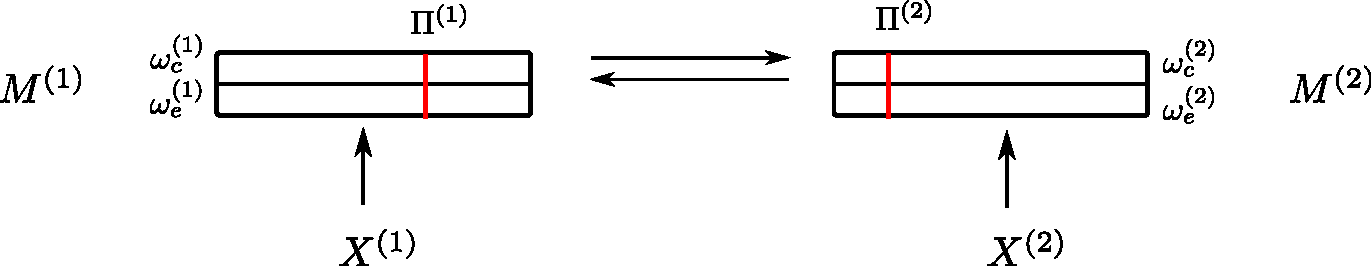
\includegraphics[width=\textwidth]{archi_2maps.pdf}
	\caption{Schéma de l'architecture de deux cartes. Chaque carte possède une couche de poids externe $\w_e$ et une couche de poids contextuels $\w_c$. Les connexions sont rétroactives~: l'entrée contextuelle de $M\m{1}$ est la position du BMU de la carte $M\m{2}$ et inversement. 
	Chaque carte prend une entrée externe $\inpx\m{i}$.\label{fig:archis}}
\end{figure}

\subsection{Modèles d'entrées et architecture de cartes}

Le modèle d'architecture étudié dans cette section est présenté en figure~\ref{fig:archis}.
Chaque carte a une taille fixée de 500 n\oe{}uds, indexés entre 0 et 1, et possède deux couches de poids $\w_e$ et $\w_c$. Les rayons de voisinage sont fixés à $r_e = 0.2$ et $r_c = 0.02$, sauf si précisé autrement dans l'expérience. Les connexions sont réciproques~: $M\m{1}$ prend comme entrée contextuelle $\bmu\m{2}$ et inversement.

Nous utiliserons comme modèle d'entrées des points en deux dimensions~: chaque modalité $\inpx\m{1}$ et $\inpx\m{2}$ correspond à l'une des deux coordonnées $x$ et $y$ de ces points. Nous comparerons la réponse de l'architecture à différents modèles d'entrées jouets générés artificiellement, qui nous permettent de maîtriser les dépendances entre les modalités.
Au chapitre~\ref{chap:repr}, nous avons représenté la dépendance entre les modalités par une variable latente $U$, en bijection avec les entrées, représentant les paramètres libres du modèle d'entrées. 
Des points 2D situés sur une courbe sont représentés par une variable $U$ 1D, et des points sur une surface par une variable $U$ 2D. L'apprentissage associatif se traduit alors par l'encodage de $U$ au sein de l'architecture.

Les modèles d'entrées que nous utilisons sont représentés en figure~\ref{fig:input_list}.
Nous reviendrons d'abord sur le modèle du cercle (\textbf{A}), qui a déjà été présenté au chapitre \ref{chap:repr}. L'intérêt d'utiliser cette courbe est que toute entrée $\inpx\m{1}$ correspond à deux valeurs possibles pour $\inpx\m{2}$ et inversement. $U$ est dans ce cas une variable 1D correspondant à l'angle du point sur le cercle.
Nous comparerons ensuite les observations réalisées sur ce modèle sur d'autres dispositions d'entrées~:
\begin{itemize}
	\item \textbf{B}~: Les entrées sont identiques.
	\item \textbf{C}~: Une entrée est une fonction de l'autre~: $\inpx\m{2} = cos(\inpx\m{1})$.
	\item \textbf{D}~: Les entrées sont sur une courbe plus complexe que le cercle, ici une courbe de Lissajous : une entrée $\inpx\m{1}$ correspond à 4 à 6 valeurs de $\inpx\m{2}$ et inversement. $U$ est une variable 1D paramétrant la courbe.
	\item \textbf{E}~:Les entrées sont totalement indépendantes, prises aléatoirement dans le patch $[0,1]^2$. $U$ est alors une variable 2D, correspondant aux coordonnées des points.
	\item \textbf{F}~: Les entrées sont sur un anneau. $U$ est alors une variable 1D, correspondant à l'angle du point sur le cercle, mais avec du bruit ajouté dans le modèle d'entrées. 
	Une carte de Kohonen classique a comme propriété d'être résistante au bruit sur les données. Ainsi, une carte 1D se dépliant sur un anneau en 2D apprendra d'abord une représentation du cercle sous-jacent. Nous voulons vérifier comment cette propriété se traduit sur l'architecture de deux cartes.
\end{itemize}

\begin{figure}
	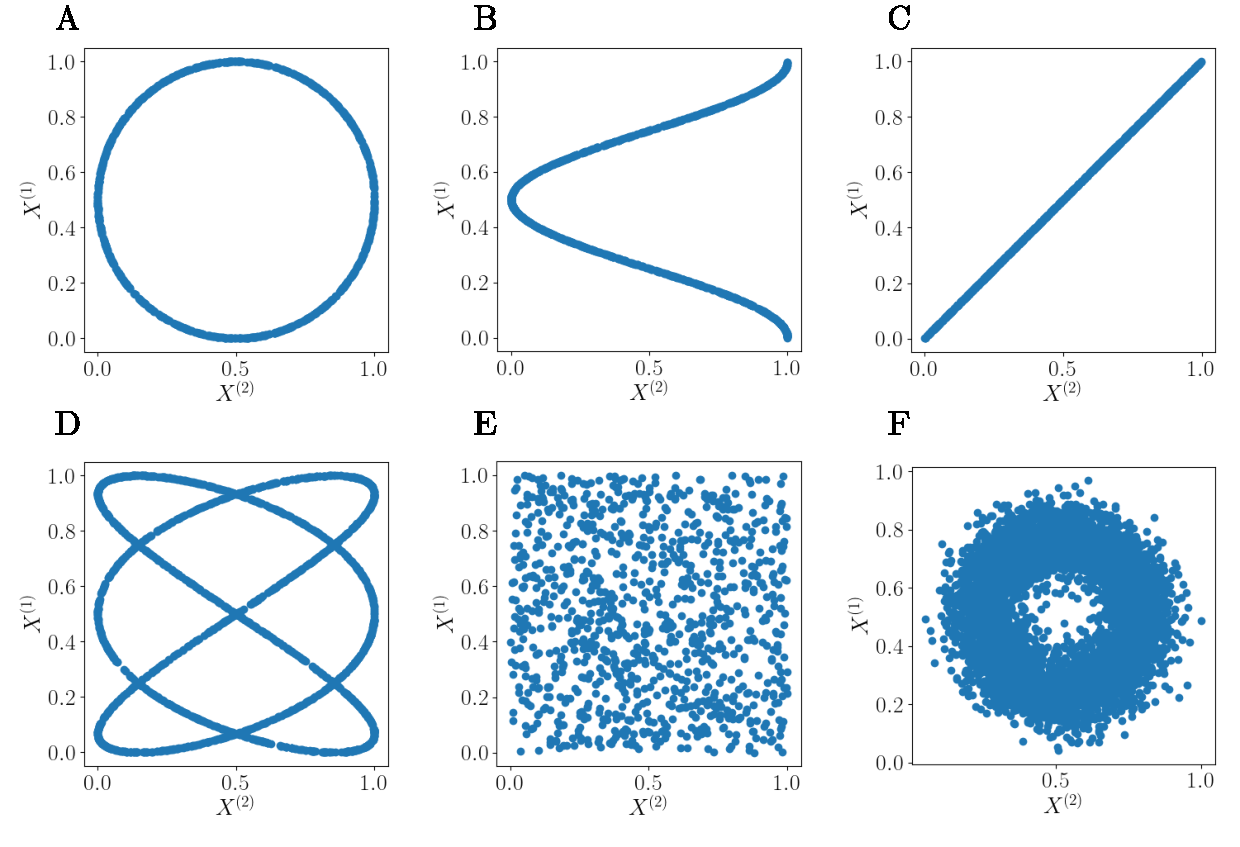
\includegraphics[width=\textwidth]{inputs/inputs.pdf}
	\caption{Dispositions d'entrées en deux dimensions utilisées dans cette section. $M\m{1}$ prend en entrée les valeurs $\inpx\m{1}$ et $M\m{2}$ les valeurs $\inpx\m{2}$. \label{fig:input_list}}
\end{figure}

Pour générer ces entrées, $U$ est tiré uniformément dans $[0,1]$, et tout couple d'entrées $(\inpx\m{1},\inpx\m{2})$ présenté à l'architecture lors de la même itération est généré à partir de la même valeur de $U$.

\subsection{Identification de mécanismes d'apprentissage sur un exemple}\label{sec:2som_cercle}

Revenons d'abord sur l'expérience sur le cercle \textbf{A}, déjà présentée au chapitre \ref{chap:repr}. 
Après avoir vérifié que les poids des cartes convergent au cours de l'apprentissage, nous détaillerons la disposition finale des poids externes et contextuels et l'organisation des BMU de la carte, afin d'identifier les mécanismes traduisant l'apprentissage des entrées et de leurs relations.

\subsubsection{Convergence des poids}

\begin{figure}
	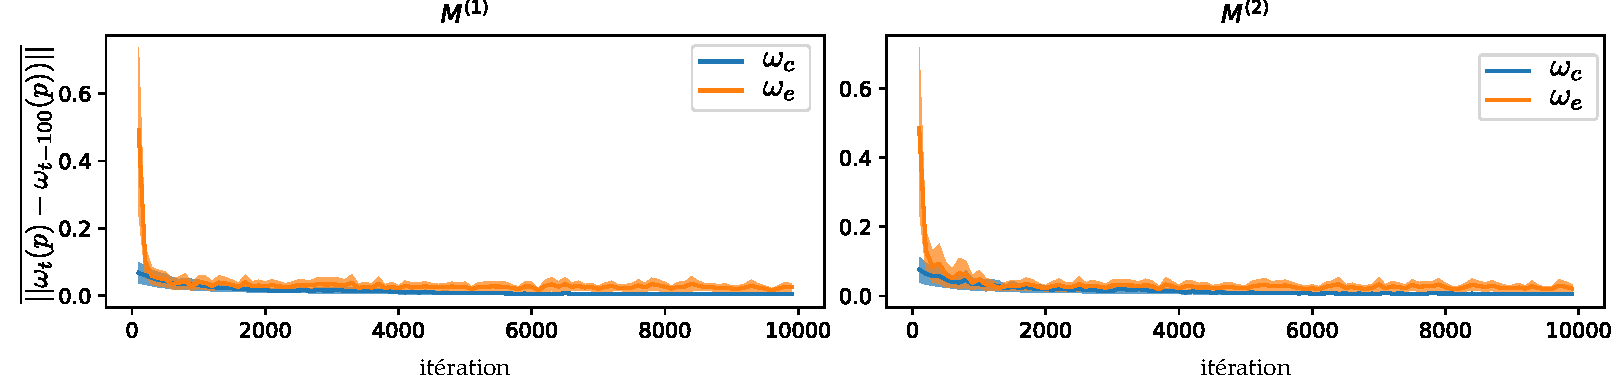
\includegraphics[width=\textwidth]{convergence/cercle_moy_2.pdf}
	\vspace{-0.5cm}
	\caption{Pour chaque carte, nous représentons l'évolution en fonction du temps de la différence moyenne entre les poids d'une carte à l'instant $t$ et ceux à $t-100$, $\langle|\w_t(p) - \w_{t-100}|\rangle$.
	L'évolution est moyennée sur 10 apprentissages dont les entrées sont tirées aléatoirement selon la même distribution d'entrées (\textbf{A}).
	Ces tracés montrent que les poids externes et contextuels évoluent rapidement vers une position dans laquelle ils ne varient plus que faiblement.\label{fig:conv}}
\end{figure}

Dans une carte de Kohonen classique, les paramètres d'apprentissage (rayon de voisinage et taux d'apprentissage) sont diminués au cours des itérations d'apprentissage. Cette diminution permet d'assurer une stabilisation des poids. Ces paramètres sont au contraire gardés constants au cours des itérations dans notre architecture, comme expliqué en section~\ref{sec:parametres_carte} p.~\pageref{sec:parametres_carte}.
Comme nous nous intéressons à l'organisation des cartes après apprentissage, nous nous assurons ici que les poids des cartes convergent effectivement vers une position stable, permettant de définir une fin d'apprentissage.
Pour illustrer cette évolution, en figure~\ref{fig:conv}, nous traçons la moyenne, sur toutes les positions $p$ d'une carte, de la différence entre $\w_t$ et $w_{t-100}(p)$~: $\langle | \w_t(p) - w_{t-100}(p)| \rangle $ à différents instants $t$ de l'apprentissage. Nous constatons que les poids évoluent rapidement au début de l'apprentissage, puis n'évoluent ensuite que très faiblement, ce qui suggère que les deux couches de poids ont atteint une position stable. Notons que ces tracés ne permettent pas de montrer expérimentalement la convergence des poids, mais donnent une bonne idée de l'évolution générale des poids des cartes.
Graphiquement, nous avons également observé que les poids évoluent vers une position stable.

Nous pouvons proposer des éléments d'explication de cette convergence observée empiriquement, en remarquant qu'une carte se comporte principalement comme une carte de Kohonen classique se dépliant sur les entrées externes. En effet, l'activité externe domine dans le calcul de l'activité globale, cf. équation~\ref{eq:global_act}.
L'activité contextuelle est utilisée ici comme un terme de modulation de l'activité externe.
La convergence des poids d'une carte de Kohonen classique en 1D sur des données numériques a été démontrée, voir~\cite{Cottrell1998TheoreticalAO}. 
La proximité du comportement de CxSOM avec une carte classique nous permet donc d'envisager que les poids des cartes CxSOM convergent également dans le cas de cartes 1D.
La convergence en l'absence de décroissance des paramètres pourrait cependant poser plus de problèmes sur des cartes en deux dimensions.

\subsubsection{Organisation de la réponse des cartes après apprentissage}

\begin{figure}
	\centering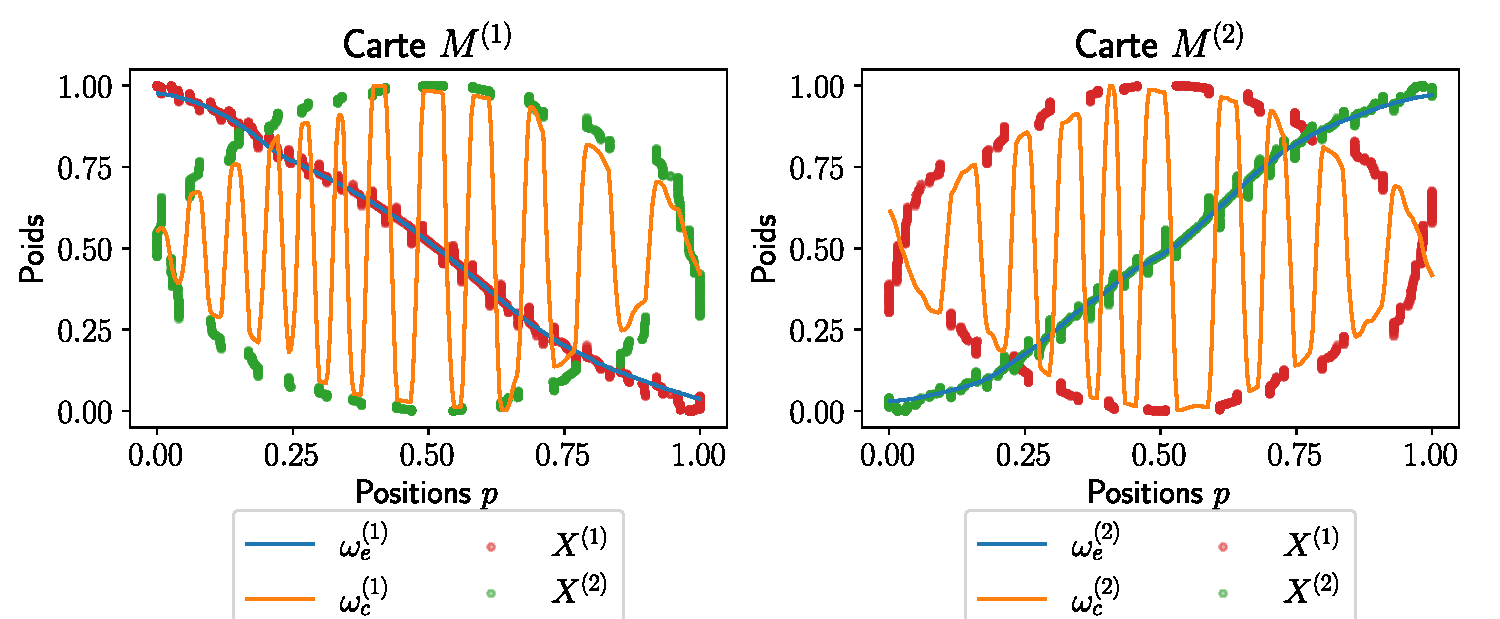
\includegraphics[width=\textwidth]{cercle/weights_500.pdf}
	\caption{Représentation cartographique des poids et entrées lors d'une phase de test selon la position du BMU dans chacune des cartes. Nous remarquons que les poids d'une carte, par exemple la carte $M^{(1)}$, s'organisent selon deux échelles. Les poids externes se déplient sur tout l'intervalle $[0,1]$, tandis que les poids contextuels forment des motifs pseudo-périodiques. 
	Les BMU s'organisent en zones, différenciant les valeurs de la paire $(\inpx\m{1}, \inpx\m{2})$ et non seulement la valeur de $\inpx\m{1}$. 
	Deux zones adjacentes codent pour des valeurs de $\inpx\m{1}$ proches, mais $\inpx\m{2}$ différents. 
	Au sein d'une même zone, les BMU s'organisent sous la forme d'une sous-carte sur les valeurs de l'entrée contextuelle. Ces zones se forment de manière auto-organisée. \label{fig:w}}
\end{figure}

Maintenant que nous avons observé que les poids convergent vers une organisation stable, nous voulons identifier comment l'organisation des poids et des BMU de l'architecture traduisent un apprentissage du modèle d'entrées \textbf{A}.
Nous avons présenté les méthodes de représentation et comparé la réponse de CxSOM à celle d'une carte simple au chapitre~\ref{chap:repr}. Nous revenons ici sur ces observations en les complétant.

Nous reprenons la représentation cartographique des valeurs d'entrées, introduite en figure~\ref{fig:inputs}. Il s'agit d'une représentation comportementale de la carte, qui permet d'observer une organisation des poids et des BMU.
Cette représentation est tracée pour les deux cartes de l'architecture en figures~\ref{fig:w} et \ref{fig:w_zoom}, après apprentissage.
Nous constatons que les poids externes, en bleu, présentent une disposition similaire aux poids d'une carte classique~: ils sont classés de façon monotone entre 0 et 1. Les poids contextuels, en orange, présentent une disposition pseudo-périodique~: ils présentent des oscillations spatiales régulières, mais les amplitudes et la largeur spatiale des oscillations varient.

La valeur des entrées $\inpx\m{1}$ et $\inpx\m{2}$ sont tracées en rouge et vert en fonction des positions de BMU obtenues lors de la phase de test.
Les positions des BMU dans les deux cartes se répartissent en zones compactes, séparées par des zones mortes de la carte dont les n\oe{}uds n'ont jamais été BMU. 
Il s'agit d'une première différence avec une carte classique, pour laquelle toutes les positions seront BMU lorsque les entrées sont distribuées de façon continue. Les zones dans lesquelles les n\oe{}uds sont BMU correspondent aux extrema des poids contextuels et leurs alentours.


\begin{figure}
	\centering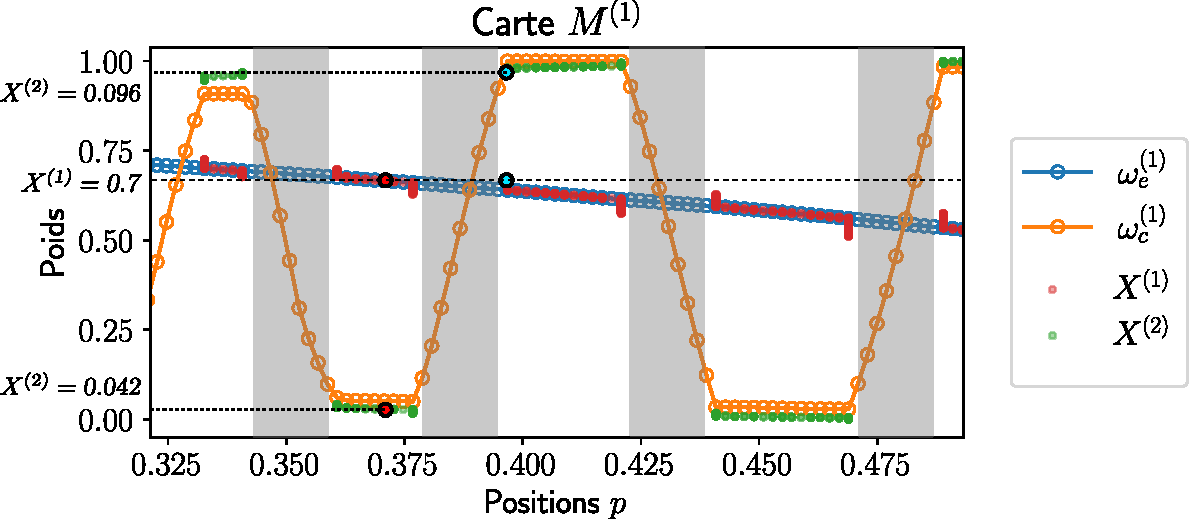
\includegraphics[width=0.7\textwidth]{cercle/weights_zoom_500.pdf}
   \caption{Zoom sur la figure \ref{fig:w} entre les positions 0.35 et 0.55 de la carte $M\m{1}$. 
   Nous y faisons apparaître la position sur la courbe des n\oe{}uds de la carte.
   Deux zones consécutives seront BMU pour des ensembles d'entrées qui se recouvrent. Par exemple, les deux entrées correspondant aux points bleu et rouge ont les mêmes valeurs de $\inpx\m{1}$, mais des valeurs différentes de $\inpx\m{2}$. Leurs BMU sont alors séparés dans la carte $M\m{1}$ dans deux zones consécutives.
   Entre les zones, quelques unités ne sont jamais BMU, en gris sur la figure. Il s'agit de zones mortes, créant des discontinuités dans la réponse de la carte.
   \label{fig:w_zoom}}
\end{figure}

La figure~\ref{fig:w_zoom} est un agrandissement de la figure~\ref{fig:w}, faisant figurer quatre zones de la carte $M\m{1}$. Elle met en évidence le fait que chaque zone de BMU (en blanc) encode un intervalle du couple $(\inpx\m{1}, \inpx\m{2})$.
Pour illustrer cette propriété, deux points sont indiqués en rouge et bleu. Ils possédent la même valeur de $\inpx\m{1} = 0.7$, mais une valeur différente de $\inpx\m{2}$. 
Ils ont ici un BMU différent dans la carte $M\m{1}$. Ces BMU sont situés dans deux zones adjacentes.
Ces tracés montrent que la réponse des cartes présente une organisation à deux échelles, portée par la forme des poids externes et contextuels. 
Dans chaque carte, le BMU est choisi selon $\inpx\m{1}$, puis localement selon $\inpx\m{2}$.
Chaque position se spécialise ainsi en fonction des deux composantes du modèle d'entrées $(\inpx\m{1}, \inpx\m{2})$. 
Chaque zone se spécialise donc pour un petit intervalle de $U$.
Nous avons ainsi observé, en section~\ref{sec:u_bmu}, que l'apprentissage des relations entre entrées se traduit par une relation fonctionnelle entre $U$ et $\bmu$ dans chaque carte, tracée en figure~\ref{fig:piu}. 
Nous reviendrons plus en détail sur cette représentation et la propriété de relation fonctionnelle entre la variable cachée et la position du BMU au chapitre~\ref{chap:indicateur}. 

\subsubsection{Erreur de quantification vectorielle}

\begin{figure}
	\centering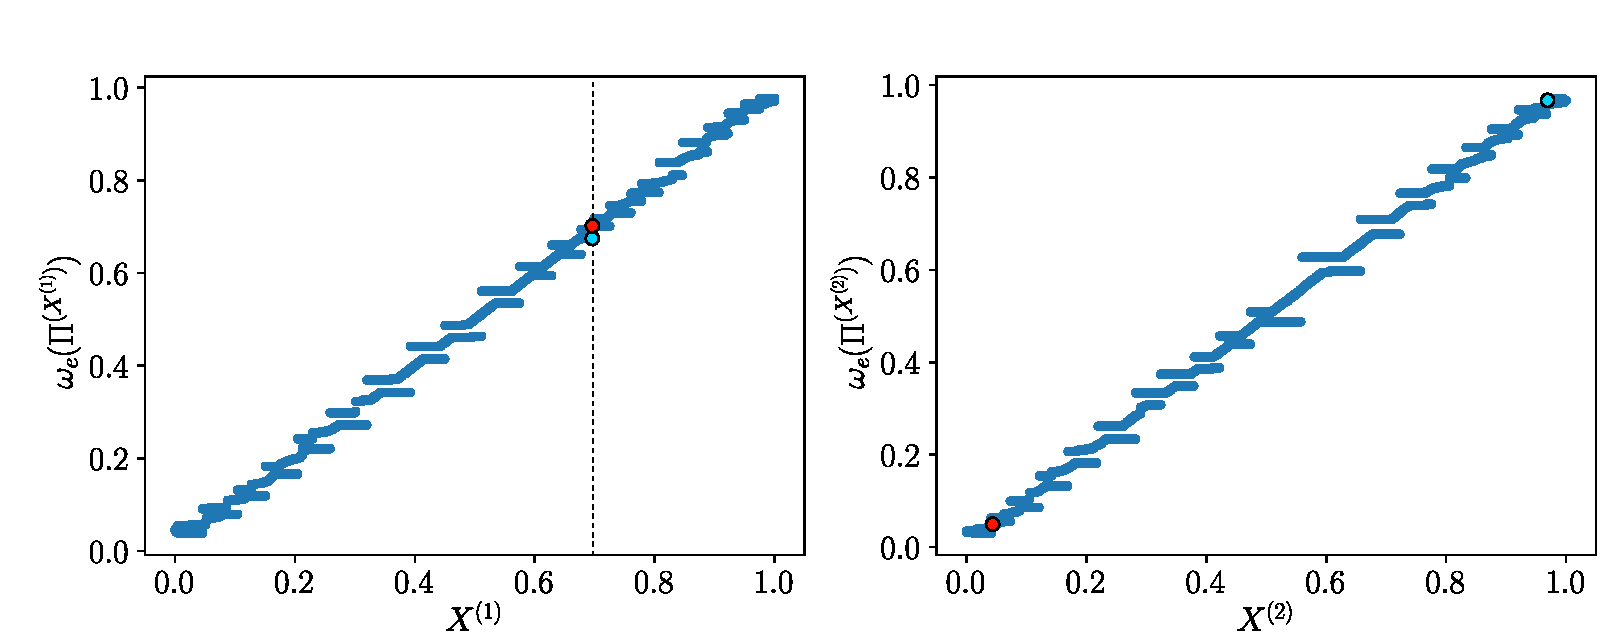
\includegraphics[width=\textwidth]{cercle/frz-error-500.pdf}
	\caption{Représentation de l'erreur de quantification sur les valeurs de $\inpx\m{1}$ et $\inpx\m{2}$. Le poids externe du BMU est proche de la valeur de l'entrée~; chaque carte réalise une bonne quantification vectorielle sur ses entrées. 
	Les mêmes points rouges et bleus représentés en figure~\ref{fig:w_zoom} sont reportés sur le graphique. Bien qu'ils aient la même valeur d'entrée $\inpx\m{1}$, leurs BMU sont placés dans deux zones de la carte. La valeur quantifiée de ces deux entrées est alors légèrement différente. 
	Ce comportement entraîne la disposition en étages observée sur le nuage de points. \label{fig:qv}}
\end{figure}

Nous nous intéressons enfin à la quantification vectorielle réalisée par la couche de poids externe sur l'entrée externe dans chaque carte. Nous souhaitons que le poids externe du BMU soit une approximation de l'entrée externe, ce qui apporte une possibilité de reconstruction de l'entrée à partir du BMU.

La figure~\ref{fig:qv} présente la valeur de cette approximation $\w\ext(\bmu\m{i})$ au sein de chaque carte en fonction de l'entrée correspondante $\inpx\m{i}$. 
Cette figure montre que la quantification vectorielle est bien réalisée~: les valeurs approximées sont proches des valeurs d'entrées.
L'erreur de quantification est néanmoins plus importante que celle qu'on obtiendrait avec une carte de même taille et mêmes paramètres apprenant sur l'ensemble des $\inpx\m{i}$. 
Nous remarquons une disposition en étages, dus aux zones formées par les poids contextuels.
En effet, une même valeur d'entrée peut avoir un BMU dans deux zones de la carte, en fonction de la valeur de l'entrée contextuelle. 
Comme les poids externes sont strictement croissants ou décroissants, cela induit l'erreur observée dans la prédiction d'entrée.

\subsubsection{Résumé des observations}

Les résultats de cette expérience ainsi que les observations présentées au chapitre~\ref{chap:repr} nous permettent de formuler les hypothèses suivantes concernant les comportements élémentaires d'apprentissage d'une architecture de deux cartes 1D~:

\begin{itemize}
	\item Les poids externes de chaque carte de l'architecture permettent à chacune d'effectuer une bonne quantification vectorielle de leurs entrées externes.
	\item Les poids externes et contextuels de chaque carte s'organisent selon deux échelles d'organisation. L'organisation des poids contextuels forme des motifs pseudo-périodiques.
	\item La réponse des cartes est marquée par la présence de zones de BMU, séparées par des zones mortes. Ces zones de BMU correspondent aux pseudo-périodes formées par les poids contextuels. Chaque zone se spécialise pour un même intervalle de valeurs du modèle d'entrées complet, donc de $U$.
	\item L'apprentissage du modèle d'entrées par l'architecture se traduit par l'existence d'une relation fonctionnelle entre $U$ et $\bmu$ dans chaque carte, montrant que chaque carte encode le modèle d'entrées et non seulement son entrée externe.
\end{itemize}

Nous cherchons dans la suite de ce chapitre à vérifier ces hypothèses sur les autres dispositions d'entrées en deux dimensions, et à compléter les observations.
Nous étudierons en particulier comment les deux échelles de quantification se forment et quelles propriétés d'apprentissage elles confèrent à l'architecture de cartes.
Nous verrons ensuite en section \ref{sec:pred} que cette organisation à deux échelles associée à la propriété de quantification vectorielle de l'entrée externe permet à l'architecture de cartes de prédire des entrées manquantes lors d'une phase de test.

\subsection{Généralisation des mécanismes d'apprentissage sur les autres modèles d'entrées}

Nous reprenons les modèles d'entrées \textbf{B},\textbf{C},\textbf{D},\textbf{E} de la figure~\ref{fig:inputs}.
Pour tous ces modèles, nous avons vérifié que la quantification vectorielle est bien réalisée dans chaque carte sur ses entrées, que nous n'avons pas tracée ici.
Nous nous concentrons sur l'organisation des poids et des BMU des cartes, afin d'identifier les propriétés d'organisation directement liées aux entrées et celles qui sont systématiques au modèle d'architecture CxSOM.

Dans la disposition d'entrées \textbf{B}, les deux entrées $\inpx\m{1}$ et $\inpx\m{2}$ sont en bijection~: une valeur de $\inpx\m{1}$ correspond à une seule valeur de $\inpx\m{2}$ dans le modèle.
La représentation cartographique correspondante est tracée en figure~\ref{fig:id_results}.
Les poids externes et contextuels s'organisent tous les deux de façon motonone entre 0 et 1. Ils sont donc sur une même échelle spatiale. Ceci s'expliquerait par le fait que la carte $M\m{1}$ n'a pas besoin de distinguer plusieurs valeurs de $\inpx\m{2}$ pour une même entrée $\inpx\m{1}$, et inversement. Les deux cartes agissent alors comme des cartes classiques, indépendantes. Leurs BMU se répartissent sur toute la carte, sans former de zones.


Dans la disposition d'entrées \textbf{C}, la dépendance entre les entrées n'est plus bijective~: $\inpx\m{2}$ est toujours une fonction de $\inpx\m{1}$, mais pas le contraire. Sa représentation est tracée en figure~\ref{fig:cos_results}.
Les poids externes et contextuels de la carte $M\m{1}$ s'organisent sur la même échelle spatiale, ce qui est cohérent avec le comportement observé sur les entrées \textbf{B}~: une seule valeur de $\inpx\m{2}$ correspond à une même valeur de $\inpx\m{1}$.
Au contraire, la carte $M\m{2}$ doit à présent distinguer deux valeurs de $\inpx\m{1}$ possibles pour chaque valeur de $\inpx\m{2}$, ce qu'elle fait en formant une deuxième échelle de quantification, grâce aux poids contextuels. Ce comportement rejoint ainsi celui que nous avons observé sur le cercle. Chaque zone de la carte $M\m{2}$ est alors spécialisée pour un intervalle de valeurs de $(\inpx\m{1}, \inpx\m{2})$ et non seulement $\inpx\m{2}$.

D'après ces deux expériences, nous supposons que la formation de deux échelles de quantification permet à une carte de distinguer plusieurs valeurs dans le modèle d'entrées qui correspondent à une même valeur pour son entrée externe. Dans ce cas, une position se spécialise en tant que BMU sur une seule valeur du modèle d'entrées.
Lorsqu'une telle division n'est pas nécessaire d'après le modèle d'entrées, les cartes s'organiseront selon leur entrée externe, de façon similaire à une carte de Kohonen classique.


Nous observons ensuite l'organisation des cartes obtenue lorsqu'une valeur de $\inpx\m{1}$ correspond à plus de deux valeurs de $\inpx\m{2}$~: 4 valeurs dans le cas de la courbe de Lissajous (Entrées \textbf{D}), tout l'intervalle $[0,1]$ dans le cas du patch $[0,1]^2$ (Entrées \textbf{E}) ou deux intervalles dans le cas de l'anneau (Entrées \textbf{F}).
La représentation cartographique est tracée pour ces trois cas en figures~\ref{fig:lissa}, \ref{fig:ind} et \ref{fig:anneau_w}.
Dans ces trois cas, les poids externes et contextuels présentent encore deux échelles d'organisation spatiale, les poids contextuels formant des pseudo-périodes.
La disposition des BMU de ces cartes forment des zones distinctes, dont chacune encode des intervalles différents du modèle d'entrées. 
Chaque zone de BMU sur $M\m{1}$ agit ici comme une sous-carte de toutes les valeurs possible de l'entrée $\inpx\m{2}$ qui correspondent aux valeurs de $\inpx\m{1}$ dans cette zone.
Par exemple, en figure~\ref{fig:ind}, chaque zone de BMU forme une carte de tout l'intervalle $[0,1]$, ce qui correspond à la distribution de $\inpx\m{2}$ lorsque $\inpx\m{1}$ est fixé.
Il est intéressant de noter que la forme des poids contextuels diffère entre toutes les dispositions d'entrées, mais que le nombre de pseudo-périodes formées par les poids contextuels reste similaire. Cette observation laisse penser que l'encodage à deux échelles est régulé par des paramètres de l'architecture, tandis que la disposition au sein des zones dépend ensuite des distributions d'entrées.

\begin{figure}
\begin{minipage}{\textwidth}
	\centering\includegraphics[width=0.8\textwidth]{id/weights.pdf}
	\vspace{-0.3cm}
	\caption{Représentation cartographique des poids et entrées pour la disposition $\inpx\m{1} = \inpx\m{2}$~(\textbf{B}). Les entrées $\inpx\m{1}$ et $\inpx\m{2}$ sont identiques, et superposées.
	Les poids externes et contextuels s'organisent selon une seule échelle spatiale.
	Les deux cartes agissent comme deux cartes indépendantes qui apprendraient sur les mêmes entrées. \label{fig:id_results}}
	\centering\includegraphics[width=0.8\textwidth]{cos/weights.pdf}
	\vspace{-0.3cm}

\caption{Représentation cartographique des poids et entrées pour $\inpx\m{2} = cos(\inpx\m{1}$~(\textbf{C}). Les poids contextuels de la carte $M\m{1}$ forment une même échelle spatiale, car une valeur de $\inpx\m{1}$ correspond toujours à une seule valeur de $\inpx\m{2}$. Au contraire, les poids de la carte $M\m{2}$ forment deux échelles d'organisation spatiale, permettant de gérer une distinction~: pour une même valeur de $\inpx\m{2}$, deux $\inpx\m{1}$ sont possibles. Les BMU s'organisent alors en zones distinctes.
\label{fig:cos_results}}


	\centering\includegraphics[width=0.8\textwidth]{lissa/weights.pdf}
	\vspace{-0.3cm}
	\caption{Représentation cartographique des poids et entrées pour des entrées sur une courbe de Lissajous, \textbf{D}.
	Comme ci-dessus, les poids externes et contextuels forment deux échelles d'apprentissage et les BMU se répartissent en zones.
	Chaque zone de $M\m{1}$ forme une carte organisée des entrées $\inpx\m{2}$ de l'architecture sur une sous-région des entrées $\inpx\m{1}$. \label{fig:lissa}}
	
\end{minipage}
\end{figure}

Nous voulons enfin observer comment est réalisée la quantification vectorielle de l'espace 2D $(\inpx\m{1}, \inpx\m{2})$ par les deux cartes. Nous prenons ici comme exemple la disposition d'entrées \textbf{E}.
En figure~\ref{fig:2som_p_d}, nous traçons la distorsion des poids externes des cartes. Il s'agit des valeurs $\omega_e(\bmu\m{1})$ en fonction de $\omega_e(\bmu\m{2})$, reliées selon l'ordre des connexions de $M\m{1}$ (à gauche) ou de $M\m{2}$ (à droite).
Nous y observons que les cartes quantifient tout l'espace $[0,1]^2$, mais par seulement 90 valeurs de ces vecteurs codes. le patch est donc seulement quantifié en 90 valeurs, ce qui est plus faible que ce que nous pourrions attendre de deux cartes ayant chacune 500 n\oe{}uds. 
Ces valeurs sont définies par les zones de poids contextuels des cartes. L'apprentissage du modèle d'entrées dans chaque carte semble ainsi réduire la capacité de quantification vectorielle sur les entrées externes.


La dernière observation que nous avions relevée sur le cercle est que $U$ est une fonction de la position du BMU dans chaque carte, ce qui montre que chaque carte de l'architecture a appris une représentation du modèle d'entrées. Le tracé de $U$ selon $\bmu$ a été effectué en figure~\ref{fig:piu} pour le cas des entrées \textbf{A}.
Nous effectuons ce tracé pour les entrées \textbf{D} (courbe de Lissajous) en figure~\ref{fig:u_bmu_lissa}. 
Cette figure fait également apparaître $U$ comme une fonction de la position du BMU dans chaque carte, ce qui étend l'observation réalisée sur le cercle.
Nous reviendrons plus en détail sur l'utilisation de $U$ dans l'analyse des réponses des cartes au chapitre~\ref{chap:indicateur}.

 \begin{figure}
 \begin{minipage}{\textwidth}
	\centering\includegraphics[width=0.8\textwidth]{square/weights.pdf}
	\caption{Représentation cartographique des poids et entrées dans le patch $[0,1]^2$, \textbf{E}. Les poids contextuels s'organisent de façon pseudo-périodique. Chaque zone de BMU définie par ces motifs forme une carte organisée des sous-régions de l'espace d'entrée externe. \label{fig:ind}}
	
	\centering\includegraphics[width=0.8\textwidth]{anneau/weights_001.pdf}
	\caption{Représentation cartographique des poids et entrées pour des entrées sur un anneau, \textbf{F}. La disposition des poids et la réponse des cartes est similaire à celle de l'architecture apprenant sur le cercle. Une architecture de cartes est robuste au bruit sur les entrées externes, ce qui étend les propriétés de robustesse au bruit d'une carte de Kohonen classique à CxSOM. \label{fig:anneau_w}}

	\hfill\begin{minipage}{0.4\textwidth}
		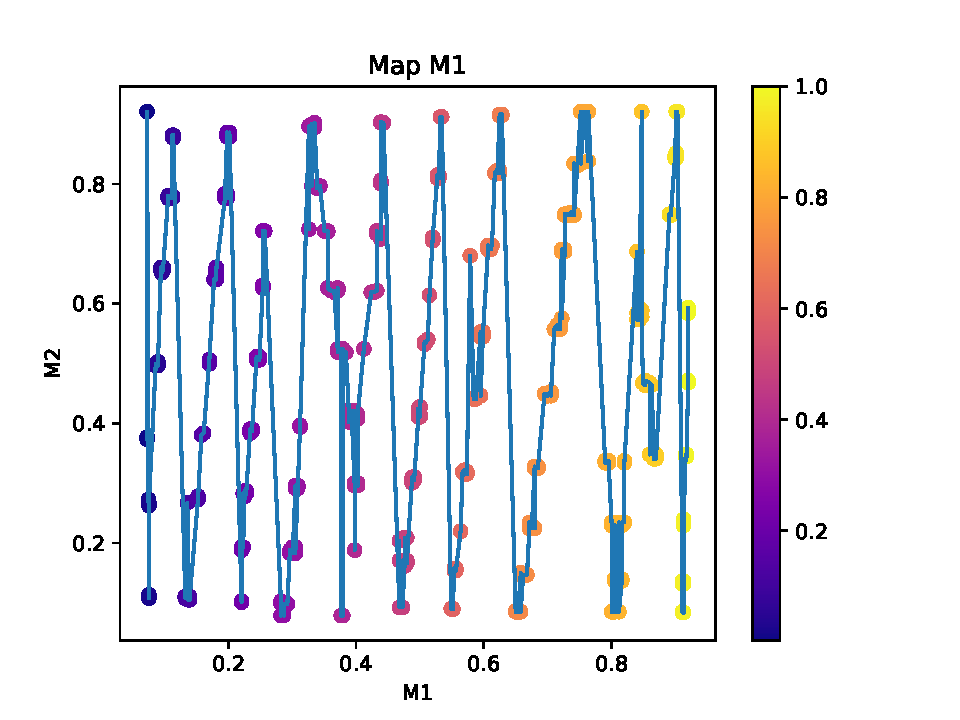
\includegraphics[width=\textwidth]{2som_square_d}
	\end{minipage}
	\begin{minipage}{0.4\textwidth}
		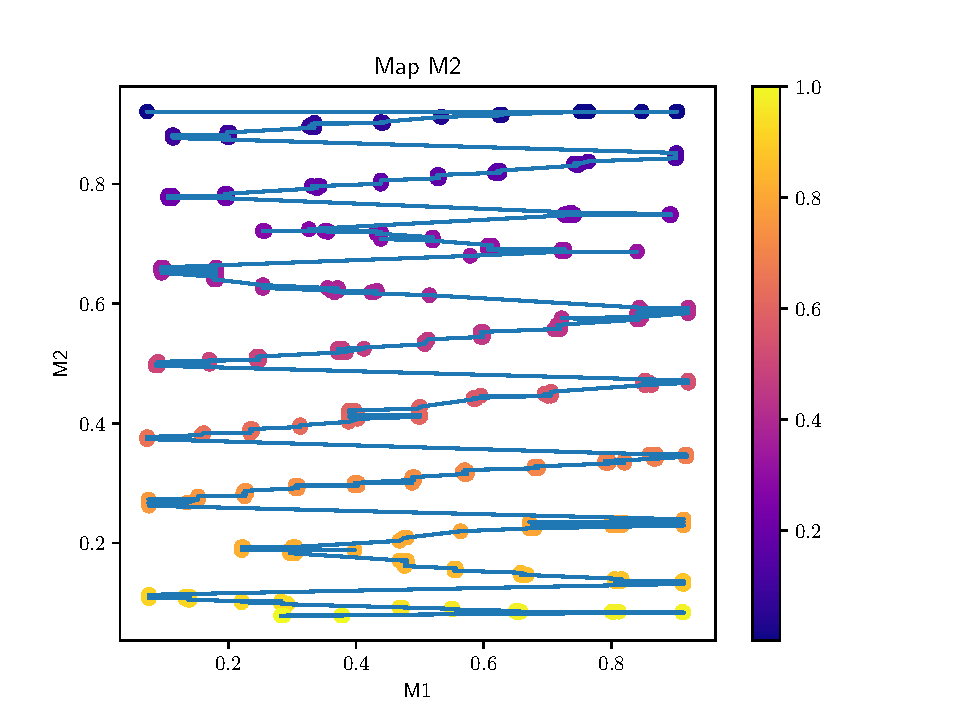
\includegraphics[width=\textwidth]{2som_square_d2}
	\end{minipage}\hfill
	\caption{Représentation de la distorsion des poids des deux cartes sur le modèle d'entrées \textbf{E}. Les cartes s'organisent de façon à représenter tout le patch $[0,1]^2$, l'une selon les $\inpx\m{1}$, l'autre selon les $\inpx\m{2}$. Bien que chaque carte ait 500 n\oe{}uds, on observe seulement environ 90 valeurs possibles des paires $\w_e(\bmu\m{1}),\w_e(\bmu\m{2})$ \label{fig:2som_p_d}}
\end{minipage}
\end{figure}

\begin{figure}[t]
	\centering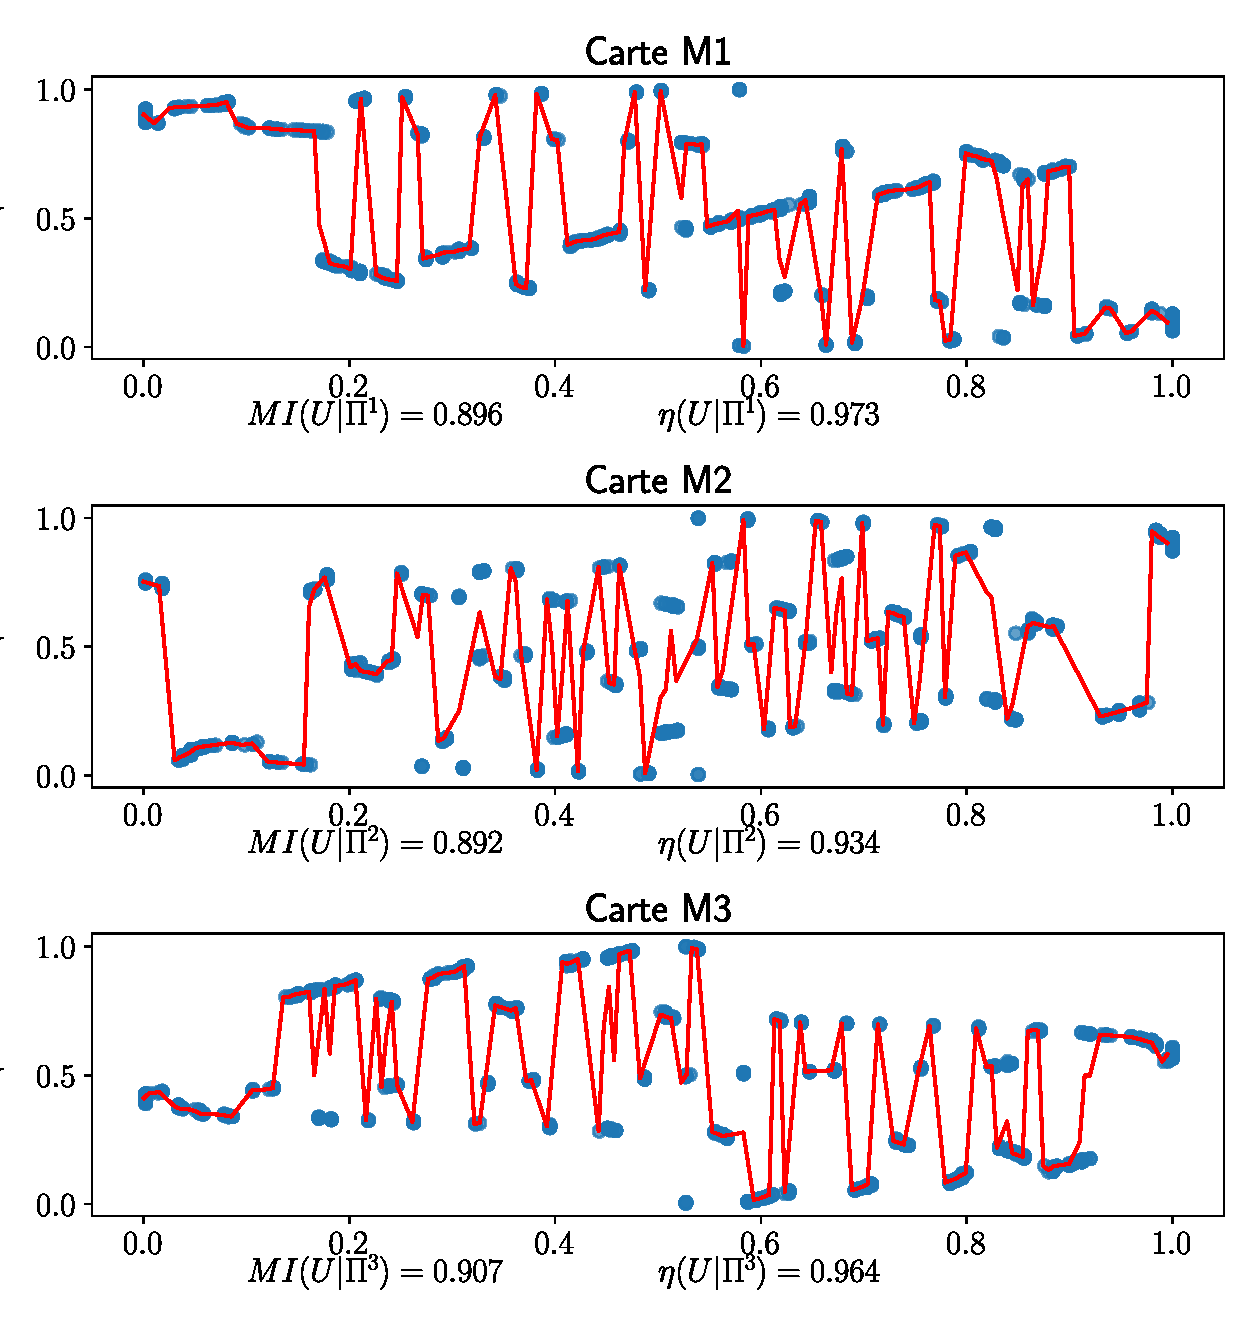
\includegraphics[width=0.8\textwidth]{lissa/U_BMU_19999.pdf}
	\caption{Représentation de $U$ selon le BMU $\bmu\m{i}$ dans chaque carte (en bleu) pour des entrées sur une courbe de Lissajous \textbf{D}. La courbe en rouge montre l'approximation du nuage de points par une fonction~: $U$ est ici une fonction de la position du BMU dans chaque carte, ce qui vérifie l'observation réalisée sur le cercle.\label{fig:u_bmu_lissa}}
\end{figure}


Grâce à ces expériences, nous postulons que l'organisation de la carte en deux échelles spatiales est un comportement systématique de l'architecture CxSOM. 
Ces deux échelles sont marquées par une organisation pseudo-périodique des poids contextuels, qui s'organisent selon une échelle spatiale plus réduite que celle formée par les poids externes. Les BMU des cartes se répartissent alors en zones distinctes, séparées par des zones mortes.
Une position de BMU se spécialise en fonction des deux entrées de l'architecture, encodant finalement une valeur du modèle d'entrées $U$. 
Une zone agit comme une sous-carte organisée, à $\inpx\m{i}$ fixé, des valeurs possible de l'autre entrée du modèle dans cette zone.

Ces deux niveaux d'indexation se forment de façon auto-organisée, mais émergent de l'organisation seulement lorsqu'il est nécessaire de pouvoir distinguer plusieurs valeurs du modèle $U$ correspondant à la même entrée externe d'une carte dans le modèle d'entrées.
Le nombre de zones reste similaire entre les expériences présentées, ce qui suggère que cette organisation est liée aux paramètres de l'architecture. La forme des zones et la réponse des cartes dépend ensuite de la relation entre les entrées.

Nous observons enfin que la quantification vectorielle globale de l'espace d'entrée choisit peu de valeurs de quantification, par rapport à ce qu'on pourrait attendre de cartes de taille 500.
Chaque carte encode donc tout le modèle d'entrées et non seulement l'entrée externe, mais au détriment de la précision de la quantification vectorielle générale des entrées. 
Ce comportement était prévisible, du fait que l'architecture possède un nombre d'unités de calcul fixé correspondant au nombre de n\oe{}uds dans les cartes.

\subsection{\'Etude des mécanismes de formation des deux échelles d'organisation spatiale}

Nous nous intéressons maintenant aux paramètres des cartes influençant la formation des deux échelles d'organisation spatiales et des zones de BMU.
Nous avons observé que la présence de zones est liée en particulier au rapport entre les rayons de voisinage externe et contextuel.
Ces paramètres contrôlent l'élasticité de chaque couche de poids.
Nous comparons dans cette section l'organisation obtenue sur plusieurs architectures ayant des couples de rayons de voisinage contextuels et externes différents, sur une même disposition d'entrée.

\subsubsection{Influence du rapport entre les rayons de voisinage sur la formation de zones de BMU}
\begin{figure}[t]
	\includegraphics[width=\textwidth]{rceqre/rcre_tot.pdf}
	\caption{Représentation cartographique de la carte $M\m{1}$ pour différents rayons de voisinage contextuels, le rayon de voisinage $r_e$ étant fixé à $0.2$. Les entrées sont tirées dans le modèle \textbf{A}.
	Nous observons que la présence de zones dépend du rapport entre les rayons de voisinage. La carte définit des zones de BMU grâce à la forme des poids contextuels. Elles sont de plus en plus nombreuses et contiennent de moins en moins d'unités lorsqu'on augmente le rapport entre rayons de voisinage.
	La carte $M\m{2}$, non représentée ici, se comporte de façon similaire.\label{fig:rcre}
	}
\end{figure}

Nous reprenons les entrées \textbf{A}, en cercle et réalisons l'apprentissage de ce modèle par plusieurs architectures dans lesquelles le rapport $\frac{r_e}{r_c}$ est différent.
Nous fixons  pour cela $r_e$ à $0.2$ et faisons varier $r_c$ de $0.2$ à $0.005$.

En figure \ref{fig:rcre}, nous traçons la représentation cartographique de $M\m{1}$ après apprentissage pour ces différents rayons de voisinages. 
Nous n'avons pas représenté $M\m{2}$, mais son comportement est semblable à $M\m{1}$ par la symétrie des entrées.
Nous constatons que la disposition des BMU en zones intervient ici pour une valeur de $\frac{r_e}{r_c} < 3$. Pour $r_c = r_e$, les poids $\w_c$ restent centrés autour de 0.5, moyennant les deux positions d'entrées contextuelles possibles pour chaque valeur de $\inpx\m{1}$.

Le nombre de zones de BMU augmente ensuite avec le rapport des rayons de voisinage. Plus il y a de zones, plus la quantification réalisée sur l'entrée externe est précise.
La taille du rayon de voisinage contextuel est  limité par la taille de la carte. Si celui-ci est trop faible, la notion de zone n'a plus vraiment de sens. C'est ce qu'on observe pour $\frac{r_e}{r_c} = 40$. $r_c$ est alors de 0.005, soit $2$ n\oe{}uds, les cartes ayant chacune 500 n\oe{}uds. 
Chaque zone de BMU ne contient plus que quelques unités, on ne peut donc plus vraiment parler de sous-carte. Néanmoins, les BMU sont toujours spécialisés en fonction des deux entrées du modèle, donc l'apprentissage associatif est toujours réalisé.

Nous verrons dans la suite du chapitre que la disposition en zones de BMU est nécessaire pour permettre l'apprentissage des relations entre entrées. Les rayons de voisinage doivent donc être choisis de façon à permettre la formation de zones. Le choix des paramètres les plus adaptés à une application restera ensuite à déterminer dans les travaux futurs~: vaut-il mieux privilégier un grand nombre de petites zones, ou peu de zones contenant de nombreux n\oe{}uds~?

Nous pouvons proposer une explication à ces deux échelles d'apprentissage par le fait que le rapport entre rayons de voisinage introduit deux échelles d'élasticités dans les poids, ainsi que deux échelles temporelles de mise à jour.
D'une part, les poids externes se déplient plus vite que les poids contextuels, car le grand rayon de voisinage externe permet de mettre à jour plus de prototypes à chaque itération.
D'autre part, les poids externes présentent une \og attraction \fg{} plus forte sur les unités voisines~: l'élasticité de la couche de poids externe est plus élevée.
Les poids contextuels doivent donc composer avec cette force. Leur organisation est ainsi subordonnée à l'organisation des poids externes. 
% Les rayons de voisinage forcent finalement les couches de poids d'une carte à s'organiser selon deux modes différents de la carte, sur leur distribution d'entrées respectives. Les poids externes sont organisés selon la fréquence $f=0$, tandis que les poids contextuels se placent sur une harmonique.


Dans nos expériences, nous avons pris des $r_c$ communs à toutes les couches de poids contextuels.
Nous pourrions cependant associer à chaque couche de poids d'une carte un rayon de voisinage différent. 
Enfin, nous pouvons aussi faire varier le taux d'apprentissage $\alpha$, ainsi que les paramètres de la fonction d'activation~: la pondération de chaque couche d'activité dans l'activation globale ou les largeurs des activations gaussiennes $\sigma$.
Pour pouvoir adapter ces paramètres automatiquement dans un objectif d'application et réaliser une étude paramétrique approfondie, il nous faudrait définir une fonction caractérisant l'organisation d'une carte, ou une fonction de coût relative à un objectif d'apprentissage. 
Nous discuterons d'un tel indicateur au chapitre \ref{chap:indicateur}, mais soulignons ici que nous n'avons pas encore défini de valeur adéquate. C'est pourquoi nous nous sommes intéressée à la compréhension de l'effet des paramètres dans nos travaux, et n'avons pas cherché à optimiser ces valeurs.

\subsubsection{Influence des deux échelles d'apprentissage sur la recherche de BMU par relaxation}
\begin{figure}
	\centering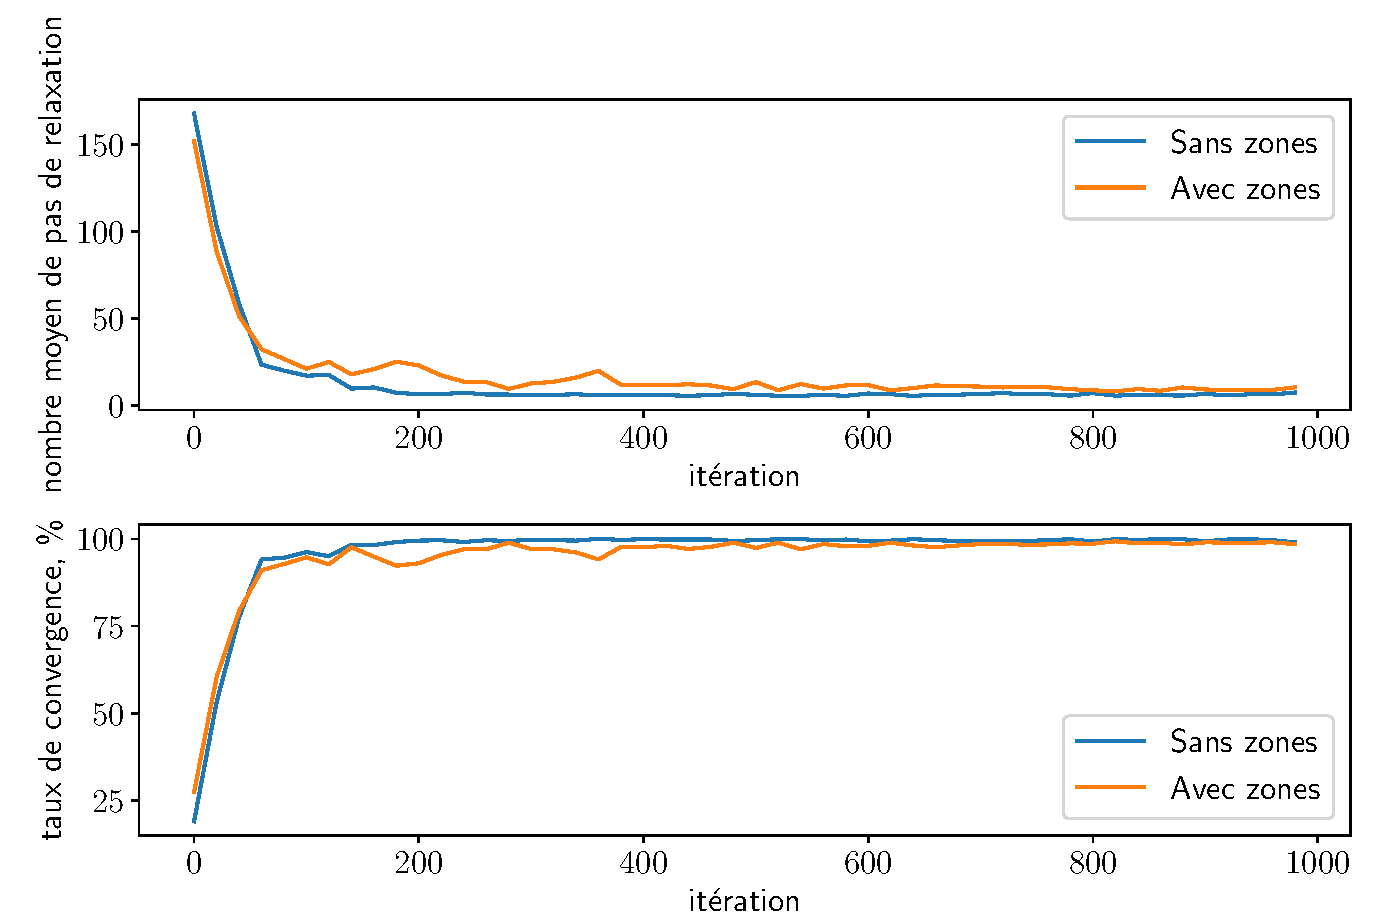
\includegraphics[width=0.8\textwidth]{rceqre/convergence_relax.pdf}
	\caption{\'Evolution du nombre moyen de pas de relaxation et du taux de convergence pour une organisation de cartes ayant formé des zones de poids contextuels ($\frac{r_e}{r_c} = 10$) et une organisation n'ayant pas formé de zones ($\frac{r_e}{r_c} = 1$). Dans les deux cas, la relaxation mène à un consensus en fin d'apprentissage. La formation de zones ne semble donc pas intervenir dans la qualité de la convergence de la relaxation. \label{fig:conv_rcre}}
\end{figure}

Nous nous interrogeons sur l'influence de la disposition à deux échelles des poids externes et contextuels dans le processus de relaxation.
Nous pouvons en effet penser que les périodes formées par les poids contextuels favorisent la recherche de consensus lors de la relaxation et la convergence des poids, ce que nous voulons vérifier ici.
Pour cela, nous comparons les indicateurs d'évolution de la convergence de la relaxation, introduits au chapitre~\ref{chap:relaxation} sur deux expériences.
Nous reprenons d'une part l'organisation obtenue en section~\ref{sec:2som_cercle}, dans laquelle les poids contextuels sont organisés en pseudo-périodes. Nous la comparons à un apprentissage réalisé sur les mêmes entrées, mais dans lequel les poids contextuels n'ont pas formé cette organisation périodique~: $\frac{r_e}{r_c} = 1$. 
Nous traçons en figure~\ref{fig:conv_rcre} les indicateurs de la convergence de la relaxation~: en haut, nous représentons l'évolution du nombre de pas moyens nécessaires à la relaxation sur une phase de test, pour des tests réalisés régulièrement au cours des 1000 premiers pas d'apprentissage.
En bas, nous traçons le pourcentage d'entrées ayant mené à une convergence de la relaxation au cours de ces mêmes phases de test, chaque phase de test contenant 1000 points.
Dans les deux cas, les phases de test en fin d'apprentissage convergent dans plus de 95 \% des cas. Cette convergence s'effectue en moyenne en une dizaine de pas de relaxation. Les deux échelles d'organisation des poids ne semblent donc pas  avoir d'influence sur la relaxation.

\subsection{Discussion}

L'observation des cartes sur ces exemples fait apparaître des motifs pseudo-périodiques formés par les poids contextuels. Ils forment une deuxième échelle d'organisation, s'ajoutant aux poids externes dont l'organisation est similaire à celle d'une carte auto-organisatrice classique qui aurait appris sur les mêmes entrées externes.
Ces deux échelles d'organisation sont un mécanisme qui émerge du processus d'évolution des cartes.
Les tracés des réponses des cartes montrent que les BMU se répartissent en zones distinctes, formées à partir des motifs de poids contextuels. Ces zones sont séparées par des zones mortes faisant office de transition et introduisant des discontinuités dans la réponse des cartes.

La formation de ces zones dépend des paramètres de l'architecture $r_c$ et $r_e$~: $r_c$ doit être inférieur à $r_e$ pour que la carte permette la formation de telles zones. 
Ensuite, leur nombre dépend surtout du rapport entre ces deux rayons de voisinage, et peu de l'organisation des entrées~: il s'agit d'une propriété induite par les paramètres de l'architecture, qui force les poids de la carte à s'organiser sur deux échelles.
Une zone correspond à un intervalle d'entrée externe~; les poids contextuels s'organisent de manière à former une sous-carte des valeurs possibles que prend l'entrée contextuelle pour cet intervalle d'entrée externe.
Finalement, chaque zone de la carte se spécialise pour un intervalle de valeur du modèle d'entrées $U$, et non seulement de son entrée externe.

\begin{figure}
	\centering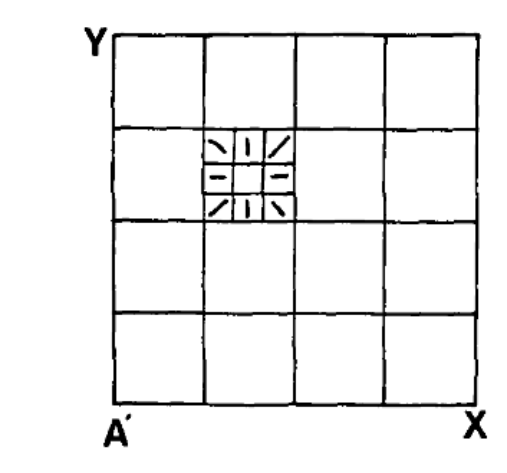
\includegraphics[width=0.3\textwidth]{ballard_primary_secondary.png}
	\vspace{-0.5cm}
	\caption{Schématisation d'une répartition en indices primaires et secondaires des neurones d'une aire corticale, tirée de~\cite{ballard_cortical_1986}. 
	Les auteurs observent que la réponse des neurones du cortex est organisée en zones selon leur position, formant des indices primaires. Les carrés de la figure représentent cette première indexation.
	Ces zones reçoivent différentes portions de l'espace d'entrée~: les zones situées à gauche du cortex traitent les signaux venant du champ visuel de gauche et ainsi de suite pour couvrir tout le champ visuel.
	Au sein d'une zone, les neurones cartographient toutes les valeurs possibles de l'entrée sous forme de carte topologiquement ordonnée, formant une indexation secondaire. \label{fig:ballard}}
\end{figure}

Cette organisation à deux échelles fait apparaître une notion d'indices primaires et secondaires dans la carte, l'indice primaire étant l'indice de la zone dans laquelle se trouve le BMU réagissant à une entrée, et l'indice secondaire la position du BMU au sein la zone.
Cette notion d'indices primaires et secondaires est également observée en biologie dans le cerveau. 
Par exemple, la figure~\ref{fig:ballard} présente un schéma d'organisation des neurones du cortex V1 décrit en \cite{ballard_cortical_1986}.
Les auteurs observent que des neurones situés à différents emplacements sur le cortex visuel ne reçoivent pas la même partie du champ de vision~; leur emplacement correspond à la partie du champ de vision traitée (gauche - droite, haut-bas). Ces entrées différenciées forment une indexation~\emph{primaire} de V1. 
Au sein d'une zone de même indice primaire, les neurones s'organisent de façon à représenter tout le sous-espace des entrées ayant été présenté à cette zone. Cette sous-carte définit alors des indices secondaires.
Dans CxSOM, la même entrée est certes présentée à toute la carte, donc la proximité avec ce modèle biologique est limitée. On peut cependant noter qu'après apprentissage, un n\oe{}ud de la carte ne réagit qu'à un sous-ensemble d'entrées définies par les valeurs des poids externes autour cet emplacement, ce qui se rapproche de ce phénomène de spécialisation d'une zone de neurones observé en biologie.


D'un point de vue des mécanismes de calcul, l'organisation d'une carte s'apparente à une technique de modulation~: la valeur de l'activité externe est modulée par l'activité contextuelle. 
Ici, la forme de poids contextuels induit une activité contextuelle pseudo-périodique, de même forme que les poids contextuels, qui vient moduler l'activité externe au sein de l'activité globale. 
L'alternance des valeurs hautes et basses dans cette activité contextuelle permet d'encoder en une même valeur, à savoir le BMU $\bmu$, à la fois l'entrée externe $\inpx$ et l'entrée contextuelle $\inpc$. Cette modulation émerge de la dynamique d'apprentissage des cartes.

\section{Génération de modalité dans des architectures de trois cartes}\label{sec:pred}

Nous avons vu que dans une architecture de deux cartes, chaque carte encode la totalité du modèle d'entrées $U$ et non seulement son entrée externe. $U$ est donc encodé dans les deux cartes de l'architecture, apportant une redondance dans l'information apprise par l'architecture sur le modèle d'entrées.

Nous voulons maintenant qu'une architecture de cartes soit directement capable d'utiliser cet encodage du modèle d'entrées dans une tâche de génération de modalité manquante après apprentissage.
Même sans qu'une entrée externe ne lui soit présentée, une carte de l'architecture possède une activité contextuelle et donc un BMU. 
Sur l'architecture de deux cartes, il est envisageable de ne pas présenter $\inpx\m{2}$ à la carte $M\m{2}$. La carte $M\m{2}$ pourra quand même définir un BMU grâce à son entrée contextuelle. 
Son poids externe $\w_e(\bmu\m{2})$ appartient à l'espace de la modalité $\inpx\m{2}$, donc la valeur $\w_e(\bmu\m{2})$ peut être considérée comme une valeur générée de cette modalité manquante.

Nous nous plaçons dans un cadre de prédiction d'une modalité manquante~: comme l'architecture a appris de l'information redondante sur le modèle d'entrées $U$, nous nous attendons à ce qu'elle soit capable de prédire une modalité qui n'a pas été présentée, à partir des autres modalités.

Dans le cas du cercle en 2D, il y a deux valeurs possibles $\inpx\m{2}$ pour une même valeur de $\inpx\m{1}$, donc il manque de l'information pour faire de la prédiction. Nous nous intéressons dans cette partie à des modèles d'entrées en trois dimensions dans lesquels la connaissance de $\inpx\m{1}$ et $\inpx\m{2}$ détermine la valeur de la troisième entrée $\inpx\m{3}$. 
Nous construirons des architectures de trois cartes sur ces deux modèles d'entrées et vérifierons la capacité de prédiction d'une modalité.
L'étude d'architectures de trois cartes nous permettra également de vérifier comment les propriétés d'organisation observées sur deux cartes s'appliquent sur une architecture de trois cartes.

Cette capacité de génération d'entrée peut constituer un cadre applicatif, par exemple lorsqu'un capteur serait manquant en robotique, ou pour donner à une carte de l'architecture un rôle de prise de décision et non seulement de réaction à une entrée. Elle permet également de valider l'encodage du modèle appris par une architecture de cartes sans avoir à connaître le modèle $U$.

\begin{figure}
	\centering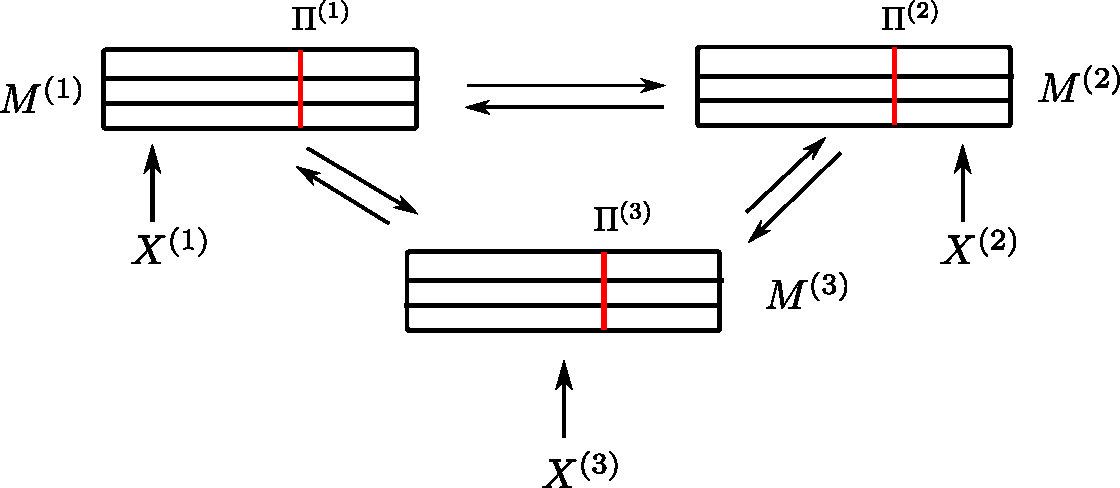
\includegraphics[width=0.6\textwidth]{archi_3maps.pdf}
	\vspace{-0.5cm}
	\caption{Architecture de trois cartes utilisée dans les expériences. Chaque carte prend une entrée externe $\inpx\m{i}$ et est connectée aux deux autres. Elle possède ainsi deux couches de poids contextuels et une couche de poids externes.\label{fig:archi_3maps}}
\end{figure}

\subsection{Méthode expérimentale}
\begin{figure}
	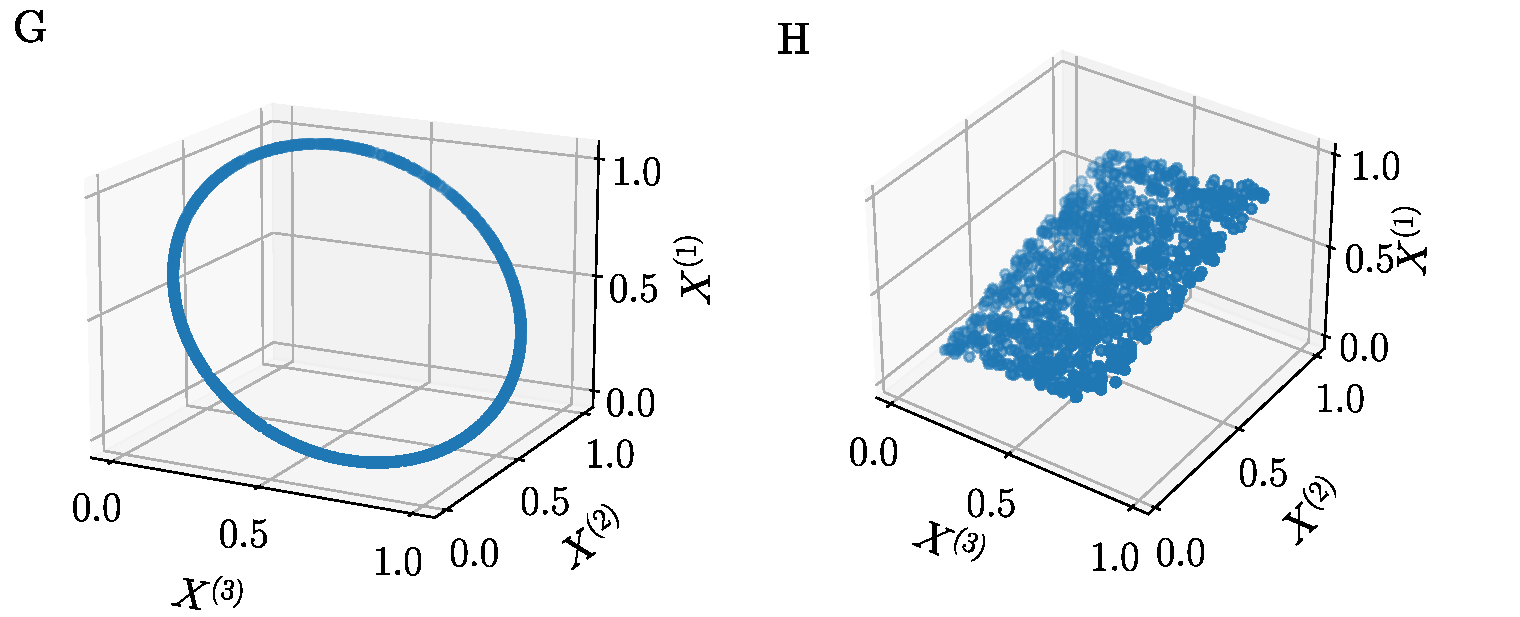
\includegraphics[width=\textwidth]{inputs/inputs_3D.pdf}
	\caption{Dispositions d'entrées en trois dimensions utilisées dans cette partie. Les entrées \textbf{G} sont sur un cercle qui a été pivoté dans l'espace en trois dimensions. Les entrées \textbf{H} sont sur un plan pivoté dans l'espace 3D.
	Chaque carte $M\m{1}$, $M\m{2}$, $M\m{3}$ prend en entrée une coordonnée $\inpx\m{1}, \inpx\m{2}, \inpx\m{3}$. \label{fig:inputs_3D}}
\end{figure}
\begin{figure}
	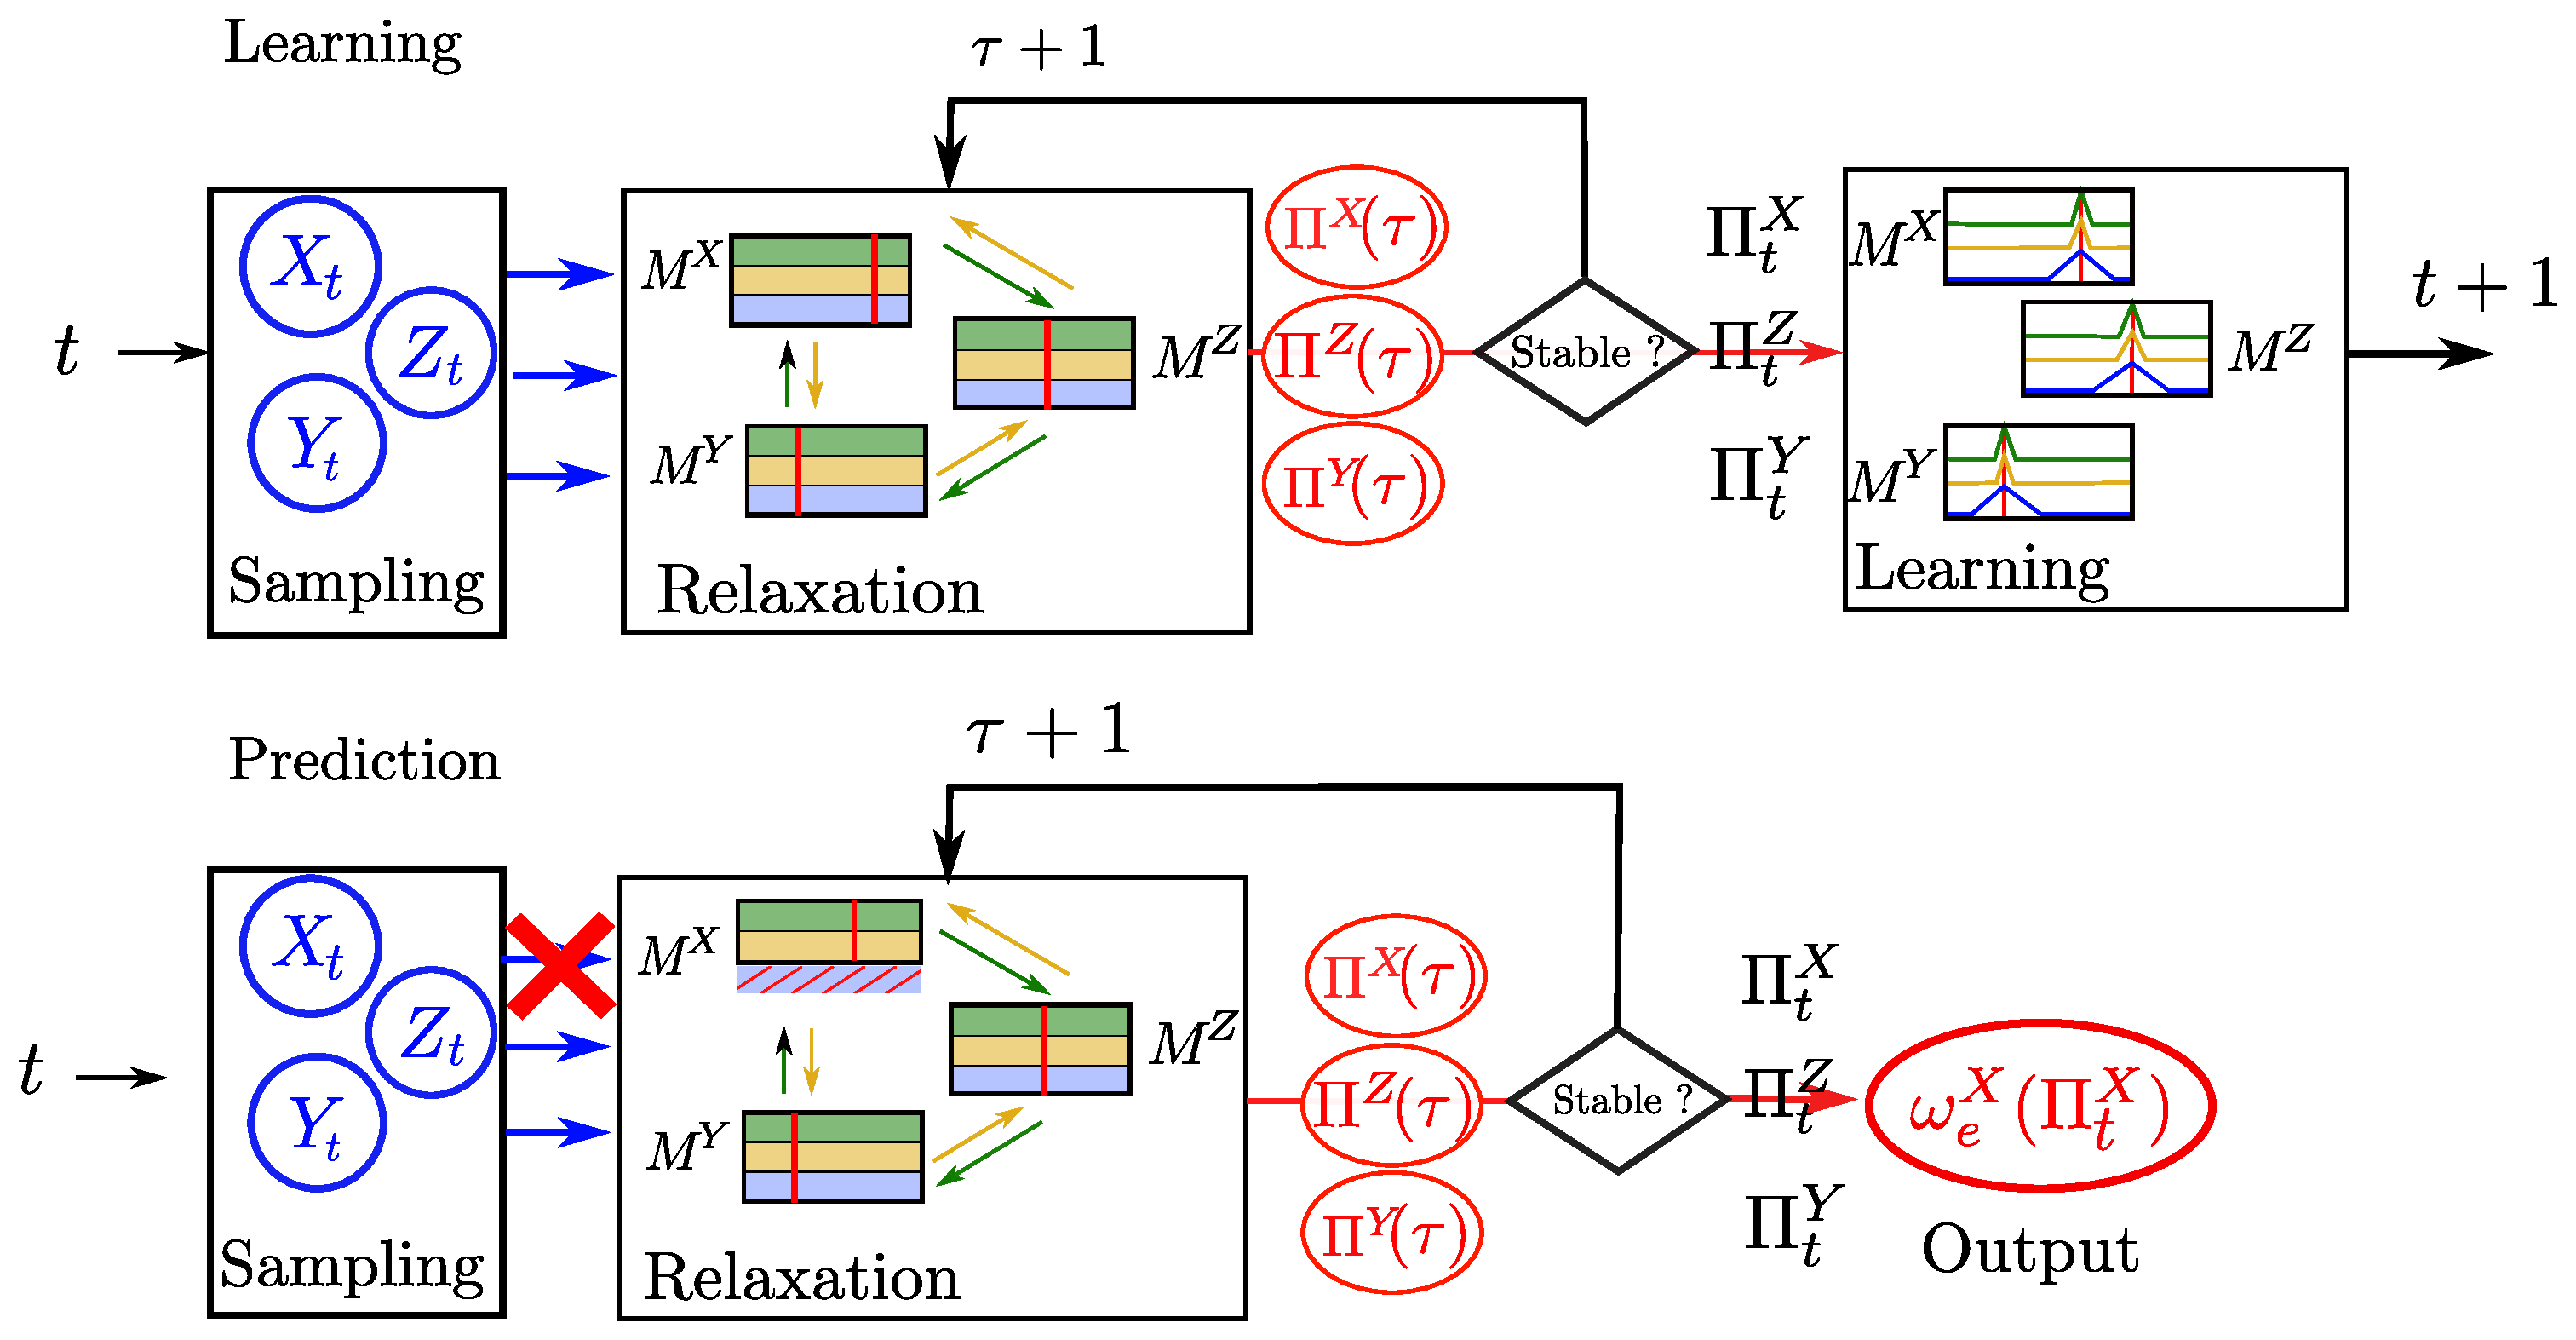
\includegraphics[width=\textwidth]{learning_tests.pdf}
	\caption{Schéma descriptif des opérations effectuées lors de l'apprentissage et de la phase de prédiction. Après une phase d'apprentissage classique, la phase de prédiction est une phase de test durant laquelle l'entrée $\inpx\m{1}$ n'est pas présentée à la carte $M\m{1}$. Celle-ci ne prend alors plus en compte d'activité externe dans le calcul du BMU par relaxation. \label{fig:schema_pred}}
\end{figure}


Les tâches de prédiction de ce chapitre seront réalisées sur une architecture de trois cartes 1D, toutes connectées entre elles~; cette architecture est représentée en figure~\ref{fig:archi_3maps}.
Chacune des trois cartes prend une entrée externe en une dimension et deux entrées contextuelles qui sont les positions des BMU des deux autres cartes. Elle possède donc deux couches contextuelles $\w_{c_0}$ et $\w_{c_1}$.
Nous construisons deux modèles d'entrées jouets à partir du cercle 2D et du patch $[0,1]^2$ en leur ajoutant une troisième dimension. Pour cela, nous pivotons le plan 2D dans lequel se situent ces entrées dans un espace en trois dimensions, de telle sorte à ce que la connaissance de deux entrées sur trois détermine la valeur de la troisième entrée. 
Ces modèles, référencés par \textbf{G} et \textbf{H}, sont tracés en figure~\ref{fig:inputs_3D}.
Chaque carte de l'architecture prend en entrée une des coordonnées des points 3D du modèle.


L'algorithme de prédiction d'entrée est schématisé en figure~\ref{fig:schema_pred}.
Lors de la phase d'apprentissage, les trois cartes reçoivent leurs entrées externes $\inpx\m{1},\inpx\m{2}, \inpx\m{3}$.
La phase de prédiction est une phase de test, durant laquelle les poids de toutes les cartes ne sont pas mis à jour.
Pour cette phase de prédiction, nous choisissons une carte, ici $M\m{1}$, comme carte prédictive, qui ne reçoit plus son entrée externe, mais seulement ses entrées contextuelles.
Les autres cartes reçoivent quant à elles leurs entrées externes $\inpx\m{2}$ et $\inpx\m{3}$.
La seule différence avec une phase de test classique est que la carte prédictive $M\m{1}$ prend comme activité globale sa seule activité contextuelle.
La valeur prédite récupérée en sortie de l'architecture est le poids externe du BMU de la carte prédictive $\w\ext\m{1}(\bmu\m{1})$.

Pour ces deux modèles d'entrées, nous vérifierons comment se traduit l'organisation à deux échelles des cartes observée en section précédente.
Nous effectuerons ensuite une phase de prédiction de l'entrée $\inpx\m{1}$ et vérifierons si la valeur prédite $\w\ext(\bmu\m{1})$ est proche de la valeur attendue $\inpx\m{1}$, qui n'a pas été présentée à la carte.


\subsection{Résultats}

Nous traçons en figures \ref{fig:w_cercle} et \ref{fig:w_plan3} la représentation cartographique des trois cartes après apprentissage, pour chacun des deux modèles d'entrées.
Nous observons d'abord que, comme pour deux cartes, les poids contextuels présentent des motifs pseudo-périodiques qui définissent une seconde échelle d'organisation au sein de la carte.
Les BMU se répartissent dans des zones distinctes. 
Les zones observées sur la représentation cartographique de $M\m{1}$ montrent que la carte choisit un BMU réagissant à $\inpx\m{1}$ de façon à différencier les deux valeurs correspondantes possibles dans le modèle d'entrées  ce qui étend le comportement observé sur deux cartes.
L'architecture ayant appris sur les entrées \textbf{H} présente également une disposition similaire à celle observée sur deux cartes.
Dans ces deux exemples, chaque carte a encodé l'ensemble du modèle d'entrées $U$, et non seulement sa seule entrée externe. L'information apprise sur $U$ est bien redondante~: nous nous attendons à ce que l'architecture soit capable de prédire $\inpx\m{1}$ à partir des seules entrées $\inpx\m{2}$ et $\inpx\m{3}$.


\begin{figure}[h!]
	\centering\includegraphics[width=\textwidth]{cercle3D/weights.pdf}
	\caption{Représentation cartographique des poids et entrées dans l'architecture de trois cartes apprenant sur le cercle en trois dimensions \textbf{G}. Les motifs pseudo-périodiques des poids contextuels et les zones de BMU sont similaires à celles observées sur l'architecture de deux cartes. Une zone encode un intervalle de valeur de $(\inpx\m{1}, \inpx\m{2}, \inpx\m{3})$. \label{fig:w_cercle}}
\end{figure}

\begin{figure}[h!]
	\centering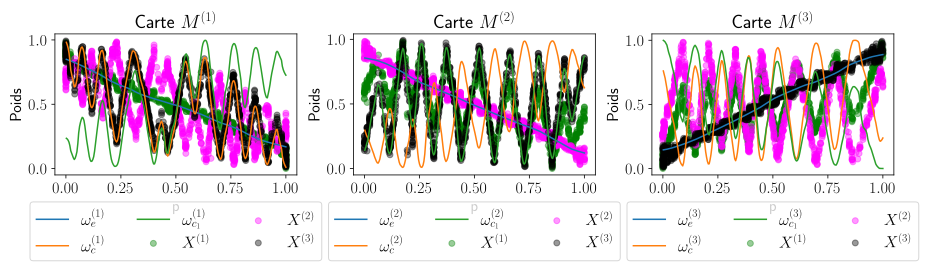
\includegraphics[width=\textwidth]{plan/weights_P2}
	\caption{Représentation cartographique des poids et entrées dans l'architecture de trois cartes apprenant sur un plan pivoté en 3D. Les zones sont similaires à celles formées par l'architecture de deux cartes. \label{fig:w_plan3}}
\end{figure}

Nous traçons l'erreur obtenue lors d'une phase de prédiction de $\inpx\m{1}$ en figure \ref{fig:pred_cercle} pour le modèle du cercle \textbf{G}, et \ref{fig:plan3_pred} sur le plan \textbf{H}.
Nous ajoutons à ces tracés l'erreur de quantification vectorielle obtenue dans les autres cartes qui ont reçu leur entrée externe lors de cette phase de test, afin de comparer la qualité de la prédiction à la qualité de la quantification vectorielle.
Nous observons que la prédiction est très bien réalisée sur les entrées tirées sur le cercle \textbf{G}. Les valeurs prédites par la carte $M\m{1}$ sont proches de l'entrée théorique $\inpx\m{1}$. Leur prédiction est aussi précise que les valeurs quantifiées par les cartes $M\m{2}$ et $M\m{3}$.
Dans le cas du plan \textbf{H}, la prédiction est également bien réalisée~: l'erreur sur la prédiction de l'entrée $\inpx\m{1}$ est équivalente à l'erreur réalisée par la quantification vectorielle dans les autres cartes.

\begin{figure}
	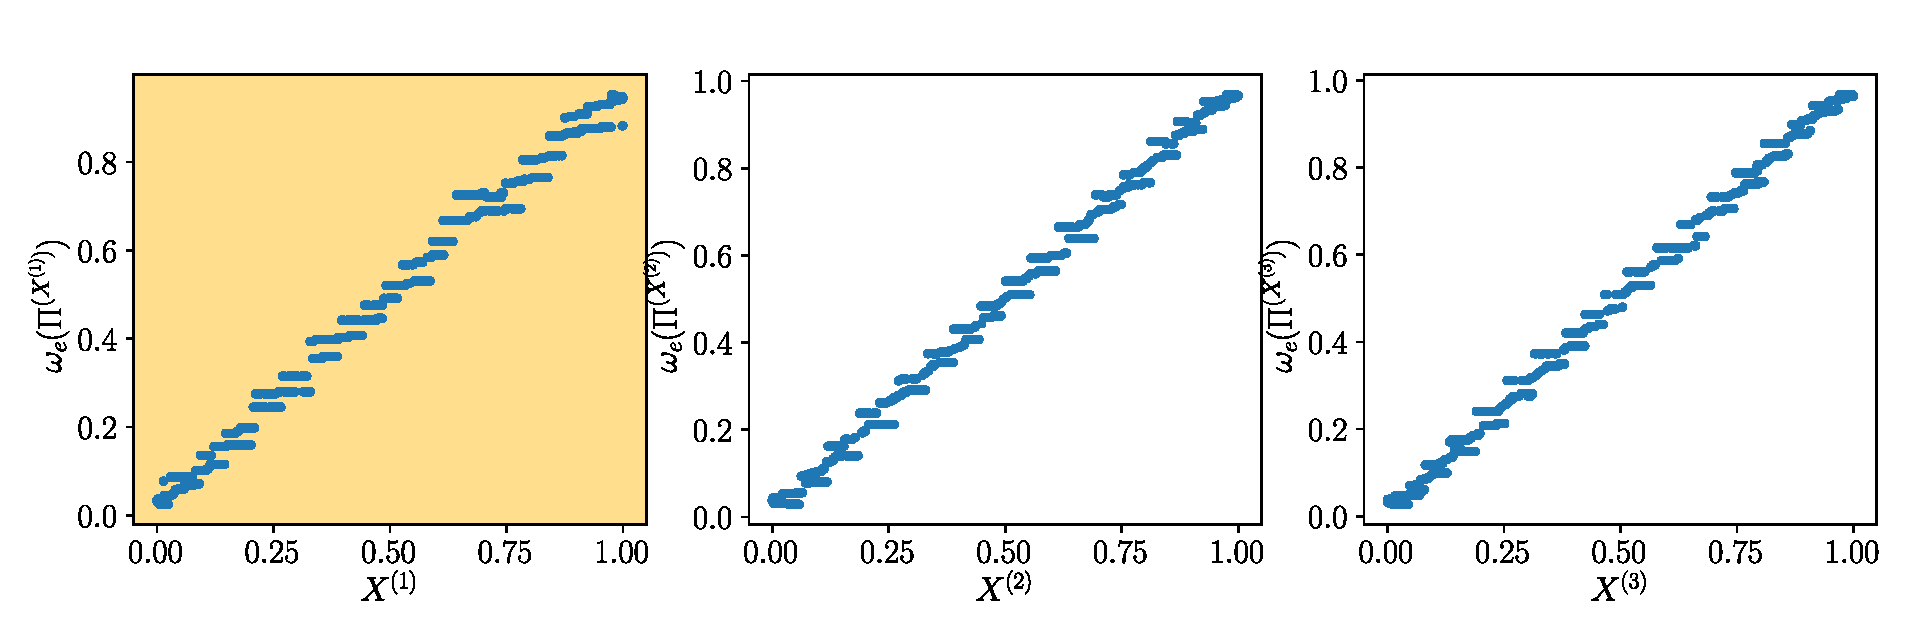
\includegraphics[width=0.95\textwidth]{cercle3D/error-closed-2.pdf}
	\caption{Erreur de prédiction de $\inpx\m{1}$ par $\w_e(\bmu\m{1})$ lorsque les entrées sont sur le cercle en trois dimensions \textbf{G}. $\inpx\m{1}$ n'a pas été présenté à $M\m{1}$.
	Les nuages de points correspondant à $M\m{2}$ et $M\m{3}$ correspondent à l'erreur de quantification dans les cartes 2 et 3 qui ont reçu leur entrée externe. Ces tracés montrent une bonne prédiction de $\inpx\m{1}$ par la carte 1. \label{fig:pred_cercle}}
\end{figure}

\begin{figure}
	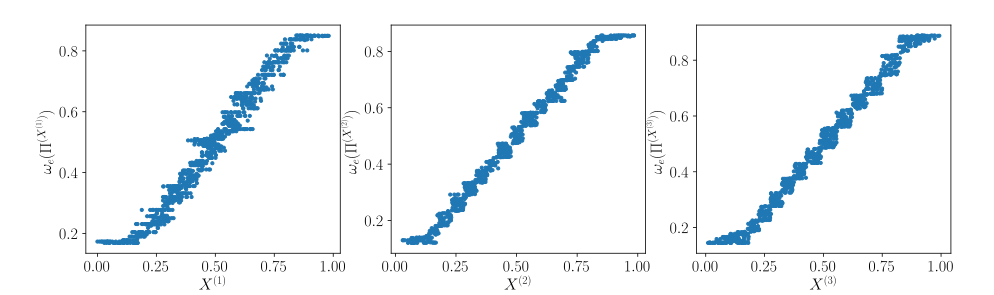
\includegraphics[width=\textwidth]{plan/zclosed-1-19999_error-P2}	
	\caption{Erreur de prédiction de $\inpx\m{1}$ dans le cas du plan \textbf{H}, montrant une bonne prédiction~: l'erreur est équivalente à la quantification vectorielle réalisée par $M\m{2}$ et $M\m{3}$. L'architecture de trois cartes est donc capable de prédire $\inpx\m{1}$. 
	\label{fig:plan3_pred}}
\end{figure}

La disposition en étages qui apparaît sur les tracés d'erreur de prédiction se rapporte directement à la disposition en zones des cartes de l'architecture.
Les entrées contextuelles reçues par $M\m{1}$ permettraient donc à une carte de sélectionner une des zones de BMU définies par les poids contextuels.
Afin de valider l'importance de cette disposition en zones dans la capacité de prédiction d'entrée, nous nous intéressons à la prédiction réalisée dans le cas ou les cartes ne se seraient pas organisés en zones.
Pour cela, nous effectuons une phase d'apprentissage et prédiction sur une architecture dans laquelle $r_c = r_e$. 
Nous avions vu que ce choix de paramètres n'engendre pas la formation de zones. L'erreur de prédiction qui en résulte est tracée en figure $\ref{fig:rcre_pred}$.
Nous observons que dans cette configuration, l'architecture de cartes n'est pas capable de réaliser la prédiction d'entrée manquante.
Bien que cette architecture ait appris les entrées externes du modèle, ne pouvons pas parler d'un apprentissage du modèle, car les cartes ne sont pas capables d'utiliser les relations entre entrées dans la tâche de prédiction.
L'organisation à deux échelles des cartes, formant des zones de BMU, permet donc bien à l'architecture de cartes d'encoder les relations entre entrées et de les réutiliser en sortie. Cette organisation est caractéristique de l'apprentissage du modèle d'entrées par l'architecture.

\begin{figure}
	\centering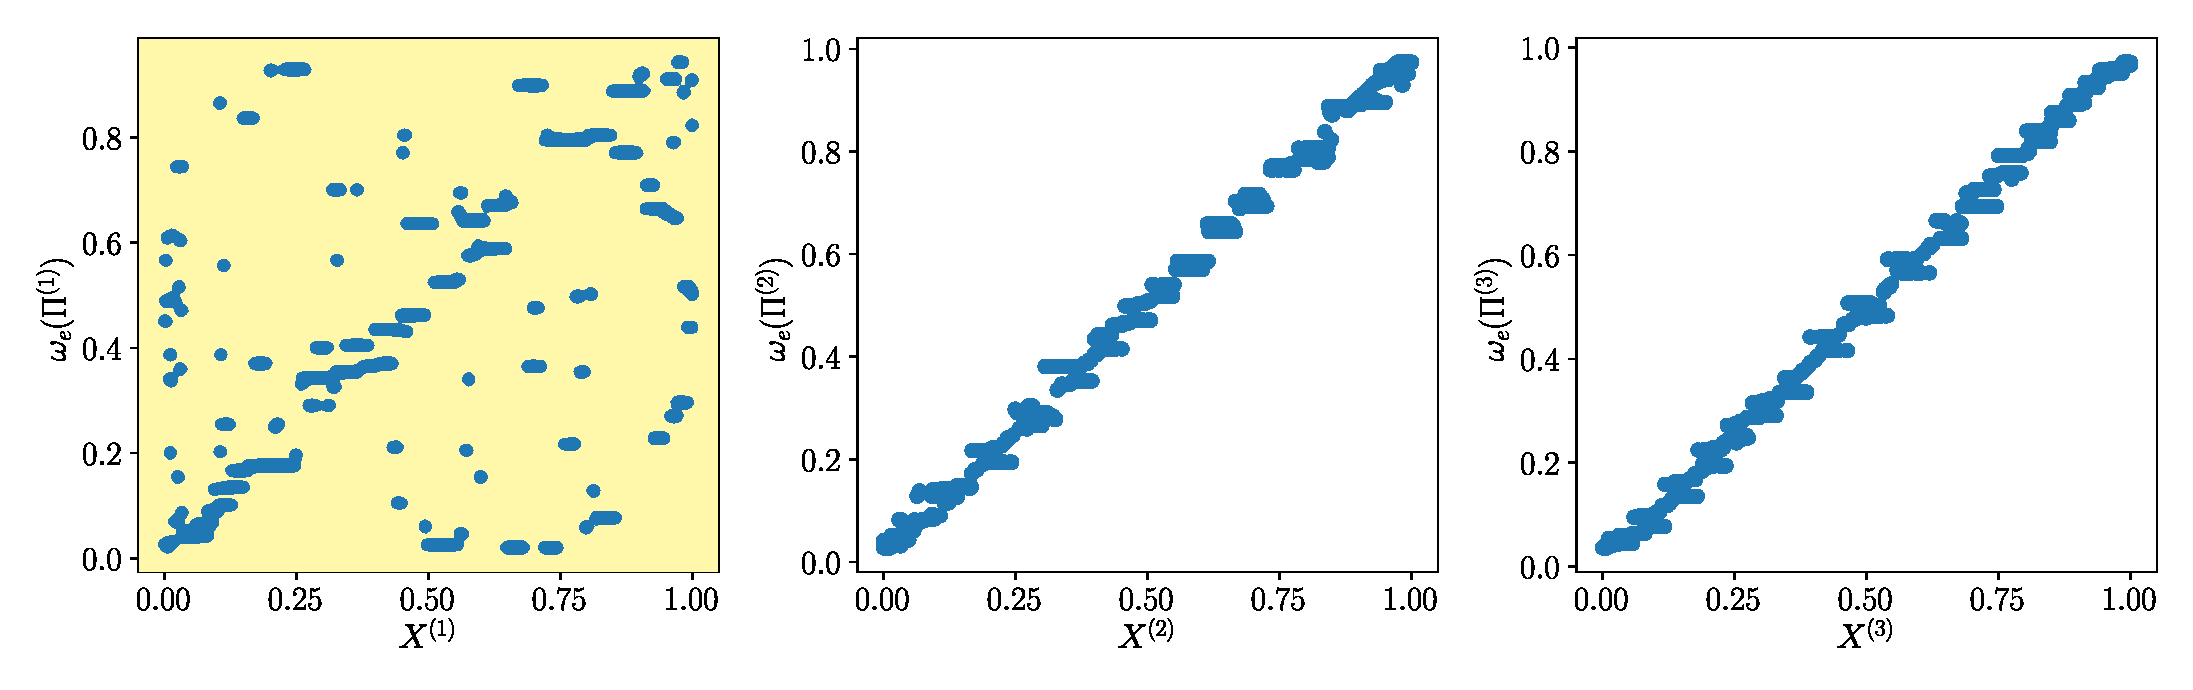
\includegraphics[width=0.9\textwidth]{rceqre/prediction.pdf}
	\caption{Prédiction de l'entrée $X\m{1}$ lorsque $r_c = r_e$. La prédiction n'est pas effectuée. Ainsi, sans formation de zones, la capacité de prédiction n'est plus réalisable par une carte de l'architecture. \label{fig:rcre_pred}}
\end{figure}

\subsection{Exemple d'application}

Nous sortons du cadre des entrées simulées pour nous placer dans un cas de contrôle réel.
Dans le cadre de travaux pratiques donnés à CentraleSupélec, nous disposons d'une plateforme expérimentale de contrôle automatique d'un drone quadricoptère.
Ce contrôle est réalisé à partir du traitement des images issues de sa caméra frontale et de ses capteurs de vitesse internes \footnote{\url{https://st5drone.metz.centralesupelec.fr/EI/visual_processing.html}}.
Cette section propose un exemple simple d'application de l'architecture en robotique en s'appuyant sur cette plateforme déjà implémentée. Cela nous permet de tester l'apprentissage d'une architecture de cartes sur des entrées bruitées, obtenues en conditions réelles et dont nous ne connaissons pas le modèle de relation.

\subsubsection{Méthode expérimentale}

\begin{figure}
	\centering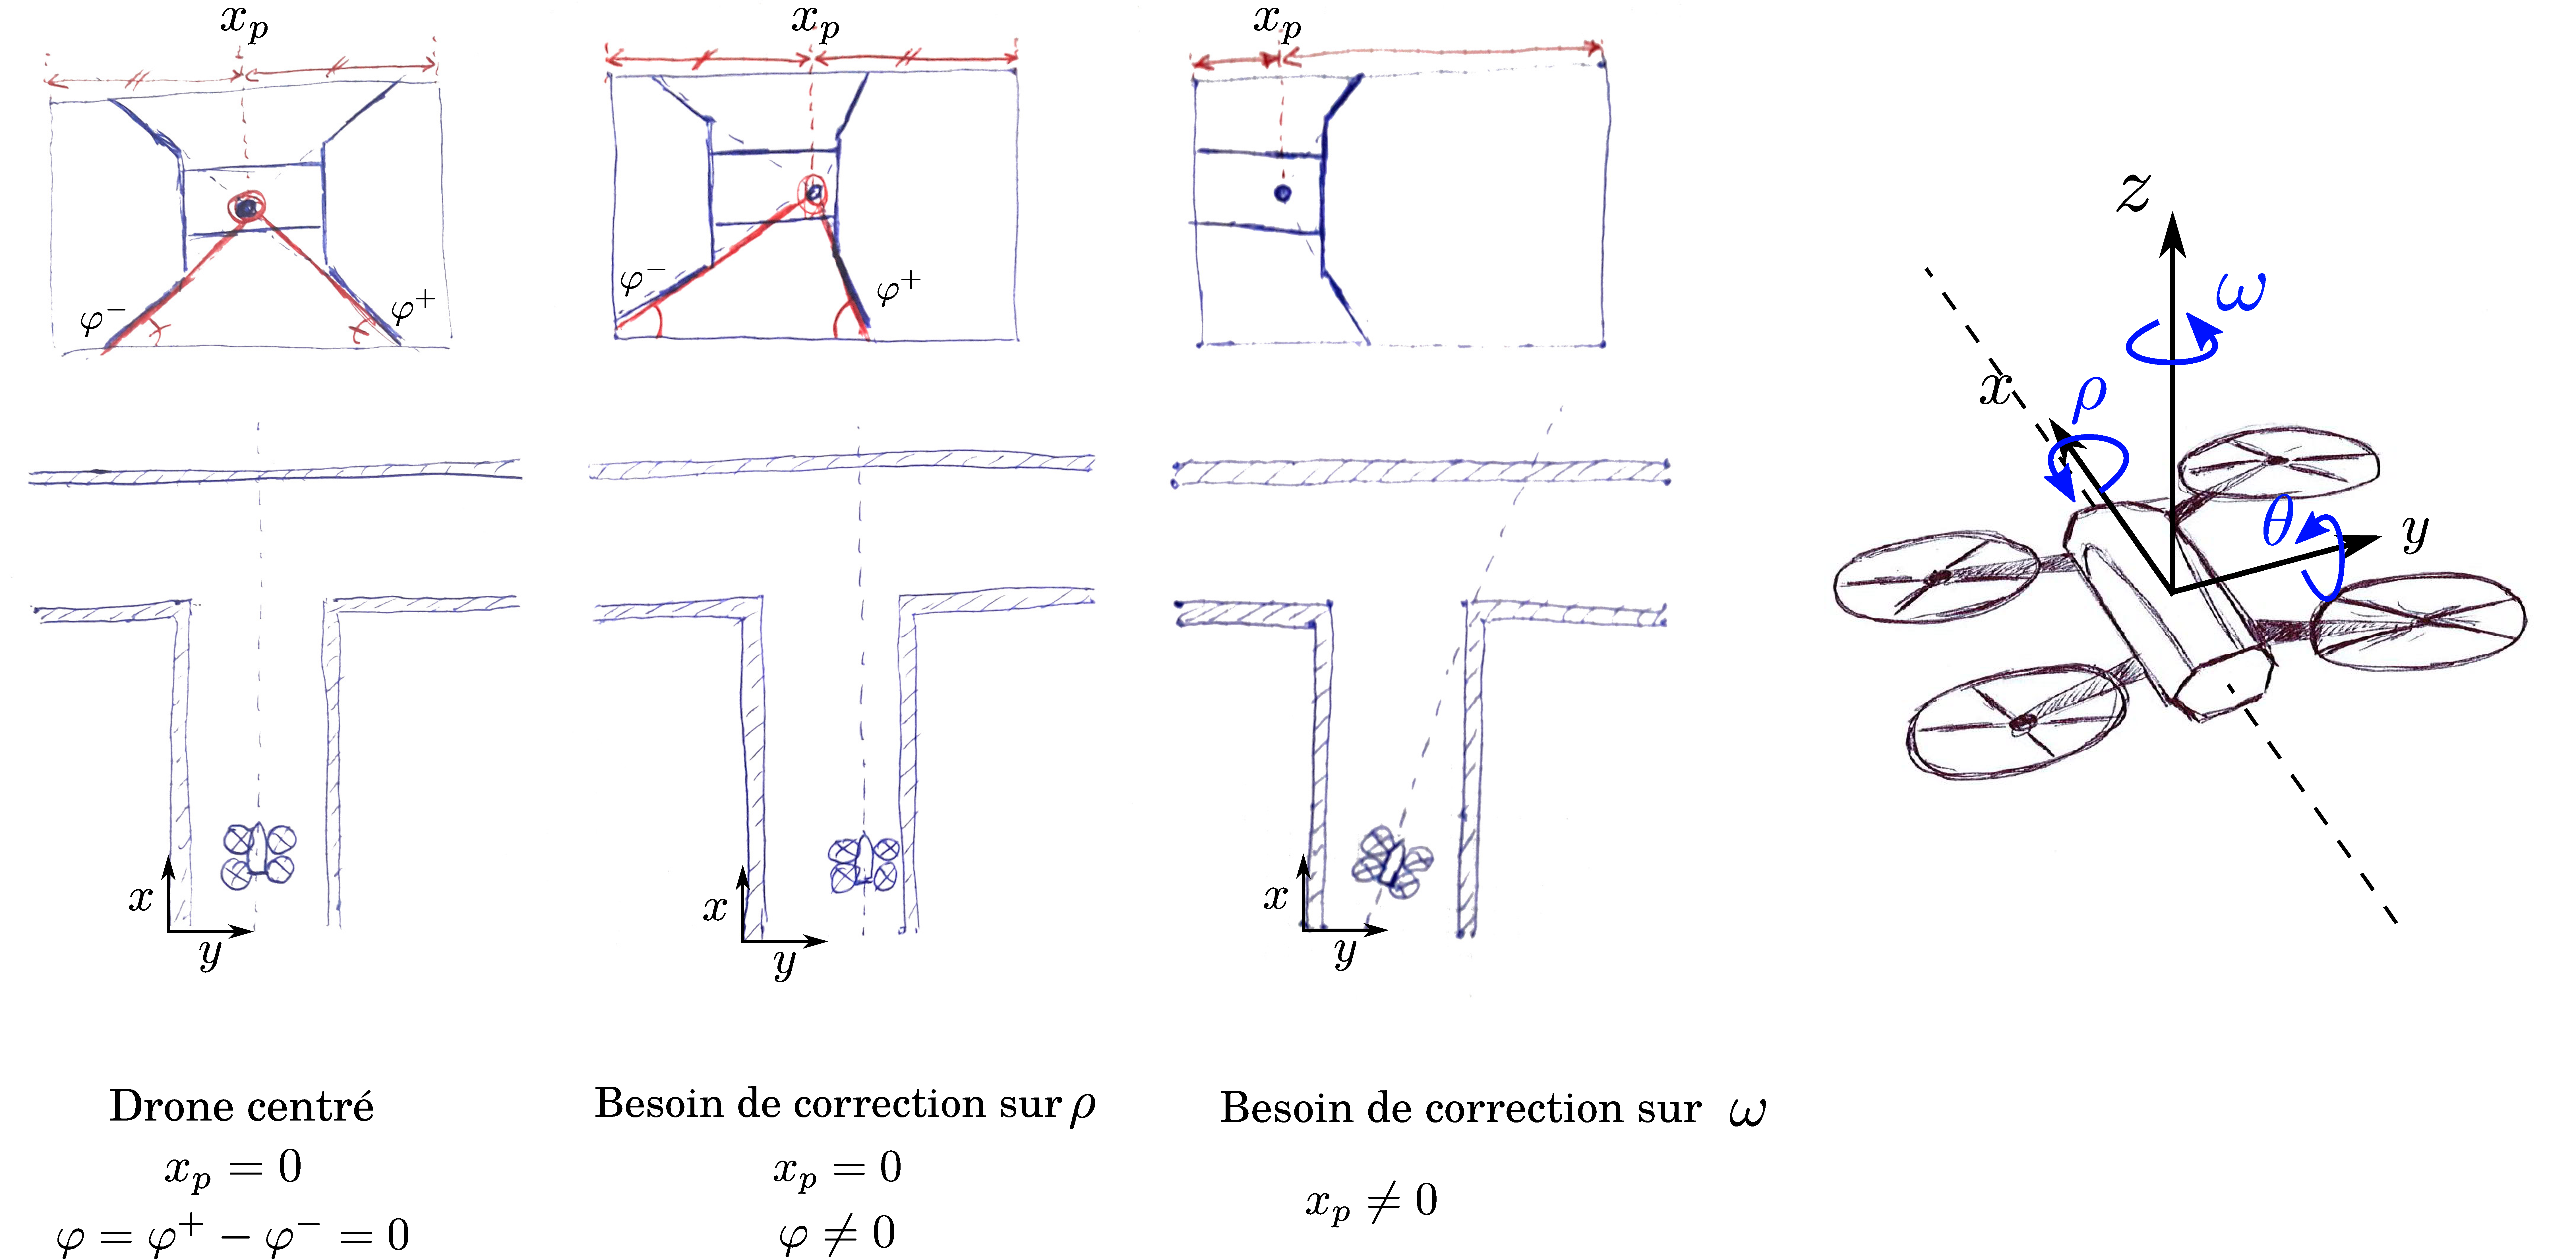
\includegraphics[width=\textwidth]{vp_drone.pdf}
	\caption{\`A gauche, représentation des situations nécessitant une correction sur la trajectoire du drone. Les images de la caméra frontale correspondant à chaque situation sont représentées en haut.
	Les commandes du drone sont représentées à droite. Il s'agit de $\w$, la vitesse angulaire autour de $z$, $\rho$, l'angle autour de l'axe $x$ (roulis) et $\theta$, l'angle autour de $y$ (tangage). 
	Pour centrer le drone dans le couloir, ces commandes dépendent de deux valeurs extraites de l'image de la caméra (en haut)~: $x_p$, abscisse du point de fuite dans le référentiel de la caméra, et $\varphi = \varphi^+ - \varphi^-$, la différence entre les angles formés par les lignes de fuite du couloir.
	Le drone vole en ligne droite lorsqu'il garde $x_p$ et $\varphi$ centrés en 0 (a).
	$x_p \neq 0$ nécessite une correction sur $\w$ (c). 
	$\varphi \neq 0$ nécessite une correction sur $\rho$ (b).
	Enfin, l'accéléromètre du drone nous permet de récupérer la vitesse linéaire du drone selon chaque axe à tout instant, $v_x,v_y,v_z$.
	}
	\label{fig:drone}
	\end{figure}

L'objectif de la tâche de contrôle est que le drone se déplace en avant en restant au centre du couloir, malgré les perturbations liées aux turbulences qu'il génère. Il possède une caméra frontale ainsi qu'un ensemble de capteurs de position et vitesse interne et peut être contrôlé à distance par un opérateur. 
% Dans le cadre du TP, la commande est asservie par des filtres proportionnel et proportionnel intégral dérivé à partir des différents capteurs et de la vitesse mesurée du robot. Cet asservissement crée une dépendance entre les capteurs du drone et les commandes à envoyer à chaque instant.
% L'idée est d'apprendre avec une architecture de SOM les relations entre les capteurs et la commande, et de remplacer l'asservissement par une prédiction de la commande.

La figure \ref{fig:drone} présente les capteurs et commandes que nous voulons utiliser pour la tâche de contrôle.
Les commandes envoyées au drone sont les angles de rotation $\theta$ (tangage) $\rho$ (roulis) et la vitesse de rotation autour de $z$, notée $\omega$. 
\`A chaque instant, nous extrayons de l'image de la caméra l'abscisse du point de fuite du couloir dans le référentiel de l'image caméra, $x_p$, et la différence entre les deux angles formés par les lignes de fuite du couloir, $\varphi$.
Pour que le drone vole en ligne droite au centre du couloir, on doit avoir $x_p = 0$ et $\varphi = 0$, ce qui correspond au cas (a) sur la figure \ref{fig:drone}.
Le centrage de $x_p$ doit être ajusté en contrôlant $\w$, par exemple dans le cas~(c).
\`A $x_p$ centré, le centrage de $\varphi$ doit être ajusté grâce à une commande sur $\rho$, ce qui correspond au cas~(b). Notons que la commande sur $\rho$ influence en fait l'accélération linéaire du drone selon $y$ à cause de la structure des hélices~: lorsque l'angle est maintenu constant, le drone accélère.


Dans le cadre du TP, nous  disposons déjà d'un programme de pilotage automatique du drone lui permettant de rester centré dans le couloir à partir de deux filtres correcteurs sur $\w$ et $\rho$.
La commande $\w$ est soumise à un filtre proportionnel à partir de $x_p$, afin de le garder centré en 0.
La commande $\rho$ influence l'accélération linéaire selon $y$.
Elle est donc contrôlée par un filtre proportionnel intégral dérivé qui permet de centrer $\varphi$ en 0, en prenant également en compte $v_y$, la vitesse linéaire selon $y$ obtenue par les capteurs d'odométrie interne du drone.
Ces deux correcteurs créent des relations, à tout instant, entre $x_p$ et $\w$ ainsi qu'entre $\rho$, $v_y$ et $\varphi$.
Nous nous retrouvons dans un cas d'entrées multimodales similaires aux entrées jouets que nous avons utilisées.
Dans notre expérience, nous voulons apprendre ces relations par une architecture CxSOM, par imitation des trajectoires contrôlées grâce aux filtres.
Nous présentons ici le résultat du contrôle de $\rho$ grâce à CxSOM, $\omega$ restant contrôlé grâce au correcteur proportionnel. L'architecture que nous avons construite cherche à apprendre les relations entre $\varphi$, $v_y$ et $\rho$, afin de remplacer la partie PID lors de la phase de prédiction. 

L'architecture CxSOM que nous avons utilisée est en fait construite sur quatre modalités~: $\varphi$, $v_y$, $\rho$ et $x_p$.
$x_p$ n'est a priori pas liée aux valeurs des autres capteurs, car contrôlée par $\w$.
Les dépendances entre ces modalités sont présentées en figure~\ref{fig:drone_inp}. Nous y voyons que $\rho$ dépend de $\varphi$ et $v_y$ de façon linéaire, mais très bruitée.
Nous connectons toutes les cartes entre elles.
 Elles ont donc chacune une couche de poids externe et trois couches de poids contextuels. Le but de l'architecture sera de capturer les relations entre les capteurs $\varphi, v_y$ et la commande $\rho$ puis de générer la commande en temps réel lors de la phase de prédiction. 

\begin{figure}
	\centering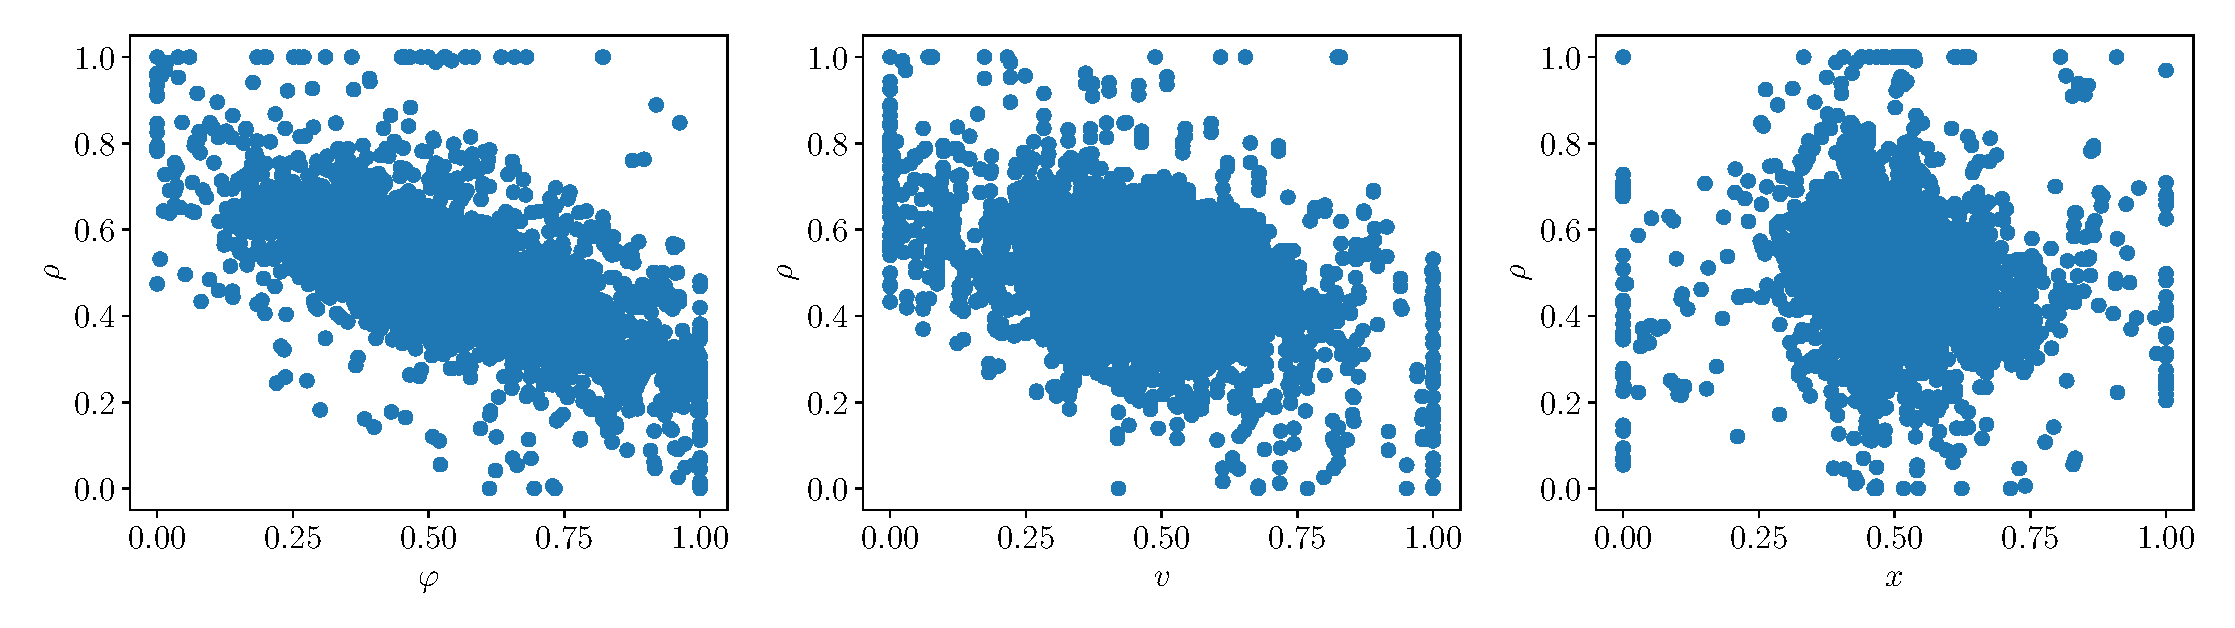
\includegraphics[width=\textwidth]{drone_inputs}
	\caption{Disposition et dépendances des entrées d'apprentissage. Nous chercherons à prédire $\rho$~: cette valeur dépend bien des autres modalités $v_y$, $\varphi$ et $x_p$. La dépendance est très simple (linéaire) mais très bruitée, et $\rho$ ne dépend pas de $x_p$. \label{fig:drone_inp}}
\end{figure}

\subsubsection{Résultats}
\begin{figure}
	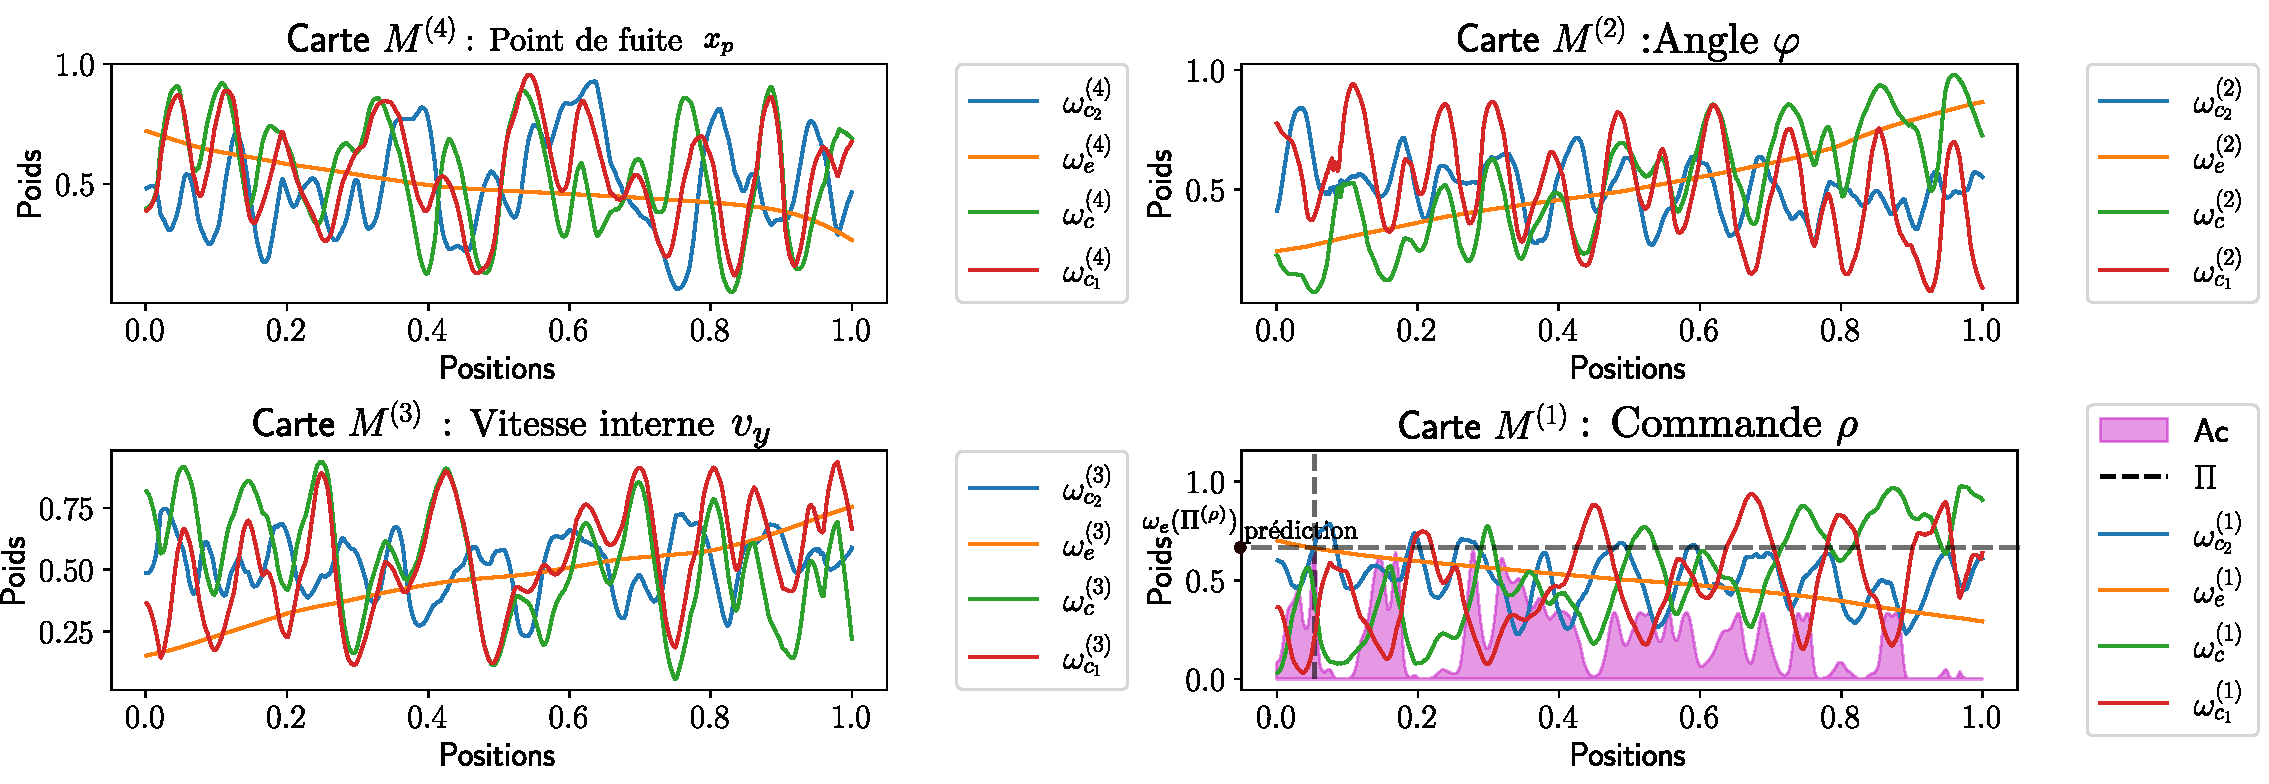
\includegraphics[width=\textwidth]{drone_weights.pdf}
	\caption{Disposition des poids des 4 cartes après apprentissage. La commande prédite $\rho$ envoyée au drone est le poids externe du BMU de la carte $\rho$, calculé uniquement à partir des activités contextuelles. Cette activité est représentée en violet sur la dernière carte.}
	\label{fig:drone_w}
	\end{figure}

	\begin{figure}
		\centering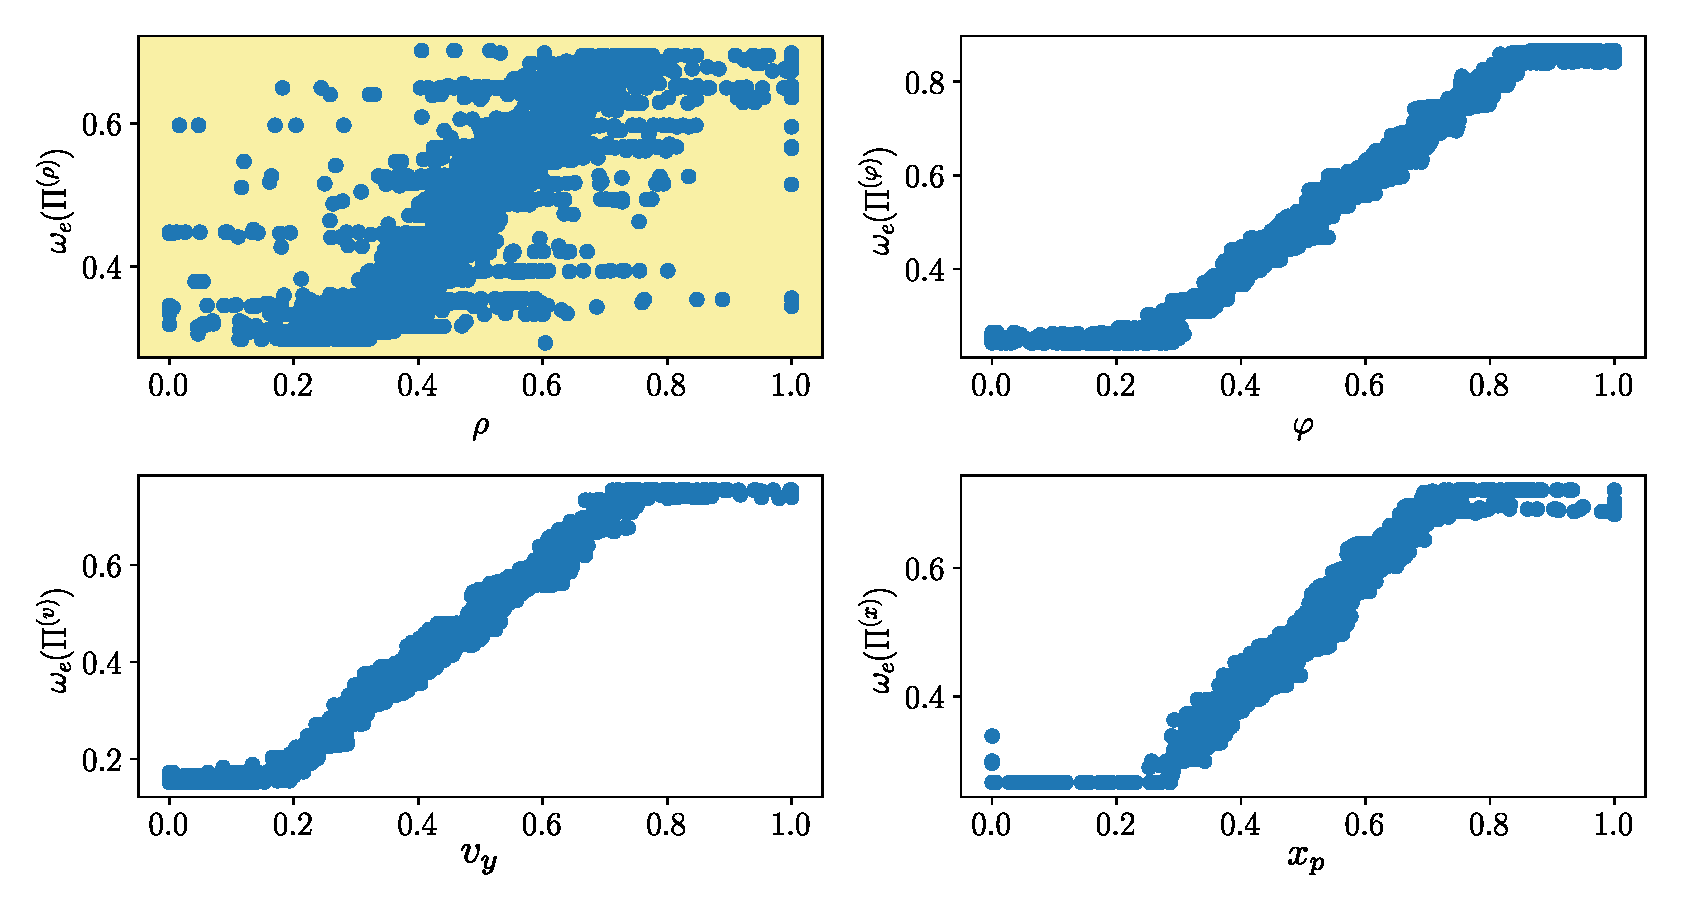
\includegraphics[width=\textwidth]{prediction_drone}
		\caption{Prédiction de $\rho$ par CxSOM sur les données d'apprentissage. Nous observons que l'entrée a été correctement prédite, bien que très bruitée, ce qui correspond aux observations réalisées en pratique. \label{fig:pred_drone}}
	\end{figure}

Les poids des cartes obtenus après apprentissage sont représentés en figure \ref{fig:drone_w}. 
Constatons d'abord que l'organisation des poids rappelle celle obtenue dans les dispositions d'entrées jouets~: les poids externes forment une cartographie ordonnée de l'entrée externe, et les poids contextuels forment des motifs pseudo-périodiques sur la carte. 
Un exemple de calcul d'activité de la carte $\rho$ pendant la phase de prédiction est illustré en violet. Le BMU correspond au maximum de l'activité~: $\bmu\m{\rho} = 0.41$ et la valeur de prédiction est $\w_e(\bmu\m{\rho}) = 0.49$. Cette valeur, remise à l'échelle, est la commande que nous envoyons au drone à l'instant $t$.
La relaxation doit être réalisée assez rapidement pour que le drone réagisse en temps réel.

Lors des expériences que nous avons effectuées, le drone apparaît voler correctement dans le couloir sans toucher les murs. Nous avons cependant constaté que cette trajectoire est très imprécise~: elle ne lui permet pas de se centrer finement au centre du couloir. Pour illustrer ce comportement, nous avons tracé en figure~\ref{fig:pred_drone} l'erreur de prédiction de $\rho$, réalisée sur les données d'apprentissage. La figure fait apparaître une prédiction très bruitée, ce qui correspond à ce que nous avons observé sur le test réel. Elle est moins bonne que la quantification des entrées réalisée dans les autres cartes. 
Au vu des relations initiales bruitées entre les modalités, nous pouvions nous attendre à une telle imprécision.

Cette application sur une architecture de quatre cartes nous permet d'abord d'étendre les observations réalisées sur deux et trois cartes~: les poids externes et contextuels forment deux échelles d'organisation, et les poids contextuels forment des motifs pseudo-périodiques dans la carte.
La capacité de prédiction laisse envisager une possibilité future d'application des architectures de cartes sur des données réelles. 
L'architecture de cartes a en effet détecté une relation entre entrées qui lui permet de prédire une commande à envoyer. De plus, la réactivité de l'envoi de la commande au drone suggère que malgré la relaxation, l'architecture réagit assez rapidement. Cependant, le dispositif expérimental réalisé ici reste à améliorer pour pouvoir envisager une réelle application de CxSOM au contrôle d'un robot. Dans ce sens, il serait intéressant d'étudier une application similaire sur des données moins bruitées et disponibles en simulation afin de mesurer l'erreur de prédiction relative à l'architecture, comme une étape intermédiaire entre les données géométriques et le cadre réel. Une telle application nécessiterait une adaptation fine des paramètres de l'architecture.
Nous pouvons imaginer, à plus grande échelle, qu'une architecture de cartes permette à un robot de réaliser une prise de décision par rapport aux valeurs reçues par ses capteurs. La capacité de prédiction laisse aussi envisager des applications relatives au remplacement d'un capteur défaillant ou à l'utilisation de données dans lesquelles il manque parfois l'une ou l'autre des modalités.

\subsection{Conclusion}

Cette section présente un comportement induit par les rétroactions dans l'architecture, à savoir la prédiction d'entrée par une carte.
Nous avons d'abord montré sur deux expériences jouets qu'une architecture de cartes est capable de générer une modalité manquante dans le modèle grâce aux connexions entre cartes. En effet, chaque carte a encodé la valeur du modèle d'entrées $U$, apportant une redondance dans l'information sur $U$ au sein de l'architecture. 
Lors d'une telle phase de prédiction, le poids externe du BMU de la carte correspondant à la modalité manquante est utilisé en tant que valeur de prédiction.
Sur les deux expériences, cette valeur est bien prédite. L'erreur de prédiction est du même ordre que l'erreur réalisée par la quantification vectorielle dans les cartes qui ont reçu leur entrée externe.
Cette capacité de prédiction est permise par l'organisation à deux échelles émergeant des cartes. L'apparition de motifs pseudo-périodiques de poids contextuels et l'organisation en zones de BMU est donc bien un marqueur de l'apprentissage du modèle par une architecture de cartes. 
Le fait que l'entrée générée corresponde directement à la valeur de l'entrée manquante vient de la quantification vectorielle sur l'entrée externe au sein de chaque carte.

Ce comportement montre que grâce à l'organisation des poids et à la recherche de BMU couplée, une architecture de cartes est non seulement capable d'encoder un modèle d'entrées, mais également de le réutiliser de façon autonome~: la génération d'entrée est réalisée par le même algorithme que celui utilisé lors des phases de tests.
Par ailleurs, les connexions d'une architecture sont rétroactives, aussi n'importe quelle carte de l'architecture peut être utilisée comme carte prédictive, ce qui constitue un avantage d'une architecture non hiérarchique.


\section{Influence des connexions sur l'apprentissage du modèle d'entrées}

Dans toutes les expériences précédentes, nous avons utilisé des architectures dans lesquelles les cartes sont toutes connectées. Or, le nombre d'architectures de cartes possibles augmente exponentiellement avec le nombre de cartes utilisées.
L'influence des connexions sur l'apprentissage d'un modèle d'entrées est donc une orientation judicieuse pour des futurs travaux sur CxSOM.
Nous présentons dans cette dernière partie deux observations ouvrant des questions sur l'influence des connexions dans une architecture.
Nous étudierons d'abord un exemple d'architecture dans laquelle chaque carte possède un grand nombre de connexions.
Nous nous intéresserons ensuite à l'influence qu'a une carte sur une autre carte qui ne lui est pas directement connectée.

\subsection{Influence d'un grand nombre d'entrées contextuelles sur l'organisation d'une carte}

\begin{figure}
	\begin{minipage}{\textwidth}
	\includegraphics[width=\textwidth]{bigdim/weights.pdf}
	\end{minipage}
\begin{minipage}{\textwidth}
	\centering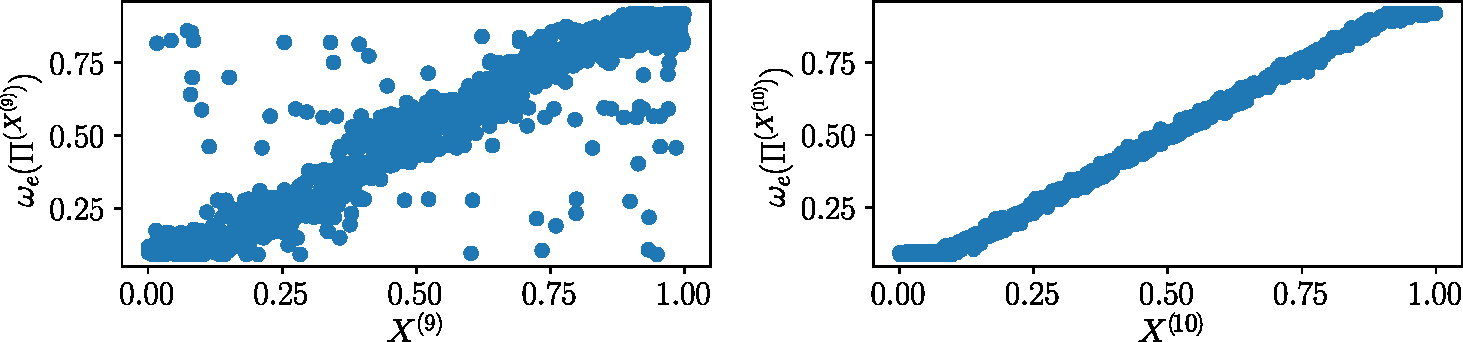
\includegraphics[width=0.8\textwidth]{bigdim/error_closed.pdf}
	\caption{En haut, tracé des poids des cartes pour une architecture de 10 cartes toutes connectées. Nous avons ici seulement tracé 4 cartes sur les 10. Les entrées sont toutes indépendantes, sauf les entrées $\inpx\m{9}$ et $\inpx\m{10}$ qui sont identiques. Les poids contextuels $\w_{c_8}\m{9}$ et $\w_{c_8}\m{10}$ correspond à la connexion entre $M\m{9}$ et $M\m{10}$.
	Nous remarquons que les poids contextuels ont évolué vers une valeur moyenne autour de 0.5, sauf ceux correspondant aux entrées dépendantes qui se sont dépliés.
	En bas, nous traçons l'erreur de prédiction de la carte 9 lorsqu'elle ne reçoit pas d'entrée. La prédiction est assez bien réalisée~: les connexions contextuelles inutiles perturbent peu l'encodage du modèle. \label{fig:bigdim}}
\end{minipage}
\end{figure}

Nous avons vu qu'une architecture de deux cartes apprenant sur le patch $[0,1]^2$ se déplie de manière à former deux échelles d'indices. 
Nous voulons étendre cette expérience pour des entrées de plus grande dimension et une architecture de plus de cartes. 
Nous choisissons d'effectuer une expérience sur 10 cartes, toutes connectées.
Nous utilisons des entrées dans l'hypercube $[0,1]^9$, et ajoutons à ces $9$ entrées indépendantes une entrée $\inpx\m{10}$ identique à l'entrée $\inpx\m{9}$. Chacune des 10 cartes prend une dimension comme entrée externe.
Nous voulons observer deux comportements~:
\begin{itemize}
	\item Comment la présence de nombreuses entrées contextuelles modifient le choix du BMU et l'organisation des cartes ?
	\item La relation entre les entrées $\inpx\m{9}$ et $\inpx\m{10}$ est-elle encodée au sein des cartes, ou cette relation est \og cachée \fg{} par toutes les connexions relatives à des entrées indépendantes ? 
\end{itemize}

La figure \ref{fig:bigdim} présente la forme des poids de quatre des cartes dans l'architecture de 10 cartes~: les cartes $M\m{9}$ et $M\m{10}$, dont les entrées externes sont identiques, et les cartes $M\m{1}$ et $M\m{2}$, dont les entrées sont indépendantes de toutes les autres entrées.
Nous pouvons noter que les poids contextuels de chaque carte présentent des motifs périodiques, rappelant ceux observés sur le plan 2D en figure~\ref{fig:ind}. L'organisation à deux échelles entre les poids externes et contextuels est donc toujours observée sur une architecture de 10 cartes.
Cependant, ces motifs sont de faible amplitude et se rapprochent tous d'une valeur moyenne constante dans chaque carte. Ces couches de poids contextuels interviennent donc peu dans le calcul de l'activité globale, et donc dans le choix du BMU. On peut supposer qu'en augmentant le nombre de connexions, les poids contextuels tendront vers une valeur constante autour de $0.5$. Dans ce cas, ils n'interviendraient donc plus du tout dans le choix du BMU.

Les couches de poids contextuels correspondant aux deux cartes dont les entrées sont identiques $\inpx\m{9}$ et $\inpx\m{10}$ sont représentées en rose dans $M\m{9}$ et $M\m{10}$. 
Elles se déplient totalement, comme nous l'avions observé en figure~\ref{fig:id_results} sur les entrées identiques. Cette couche de poids sera ainsi la seule à réellement intervenir dans le choix du BMU. L'architecture de 10 cartes a donc encodé la relation existant entre $\inpx\m{9}$ et $\inpx\m{10}$ malgré les autres connexions contextuelles inutiles.
En bas de la figure, nous traçons également la prédiction de l'entrée $\inpx\m{9}$.
Cette prédiction est correctement réalisée, bien que plus bruitée que dans le cas d'une seule connexion~: les connexions inutiles perturbent peu l'apprentissage des relations entre entrées. 
Finalement, les cartes $M\m{9}$ et $M\m{10}$ ont appris à effacer du calcul de l'activité les entrées indépendantes de leur entrée externe, et gardé les entrées contextuelles qui ont une relation avec leur entrée externe.

Cette expérience propose une idée de comportement à grande échelle à explorer plus en détail.
En particulier, on peut se demander si ce comportement peut permettre d'extraire automatiquement des relations entre entrées. Cette détection de relations serait une possibilité de comportement émergent d'une grande architecture de cartes.

\subsection{Influence des connexions distantes sur l'organisation d'une carte}
\begin{figure}
	\centering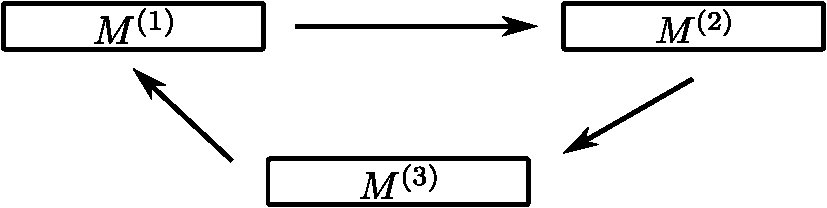
\includegraphics[width=0.5\textwidth]{loop/archi.pdf}
	\caption{Schéma de connexions d'une architecture en \og boucle\fg{}. \label{fig:archi_loop}}
\end{figure}

Nous cherchons maintenant à observer comment une carte d'une architecture peut influencer une carte qui ne lui est pas directement connectée.
Dans cette deuxième expérience, nous repassons sur une architecture de trois cartes 1D et reprenons comme modèle d'entrées le cercle en trois dimensions (\textbf{G}). 
Nous voulons comparer le comportement d'une architecture dans laquelle les cartes sont connectées réciproquement, présentée plus haut, à celui d'une architecture de trois cartes connectées en boucle, dans laquelle chaque carte est uniquement connectée à une seule autre carte. 
Ce modèle d'architecture est illustré en figure~\ref{fig:archi_loop}~: $M\m{1}$ nourrit $M\m{2}$, $M\m{2}$ nourrit $M\m{3}$ et $M\m{3}$ nourrit $M\m{1}$.

La disposition des poids de cette architecture après apprentissage est tracée en figure~\ref{fig:3som_loop}.
Les poids des cartes montrent une organisation similaire au cas où les connexions sont réciproques, cf. figure~\ref{fig:w_cercle}. Les poids contextuels forment des motifs pseudo-périodiques, et chaque carte différencie ses BMU en fonction du modèle d'entrées $U$ et non seulement de son entrée externe.
D'après les éléments d'étude que nous avons établis précédemment, nous pourrions donc dire que l'architecture a encodé le modèle d'entrées dans chaque carte.

Nous nous demandons si cette architecture en boucle est capable de prédire $\inpx\m{1}$. 
La carte prédictive $M\m{1}$ ne reçoit alors que l'entrée venant de $M\m{3}$~: $M\m{2}$ intervient seulement de façon distante dans le calcul de l'activité de $M\m{1}$.
Afin de dissocier l'influence de $M\m{2}$ et $M\m{3}$ dans la prédiction de $\inpx\m{1}$, nous réalisons également une phase de prédiction effectuée uniquement à partir des cartes $M\m{3}$ et $M\m{1}$, sur les mêmes dispositions de poids que dans l'architecture en boucle.
Dans le premier cas, $M\m{2}$ contribue à la prédiction via $M\m{3}$~; elle n'intervient pas dans le second cas.

\begin{figure}
	\centering\includegraphics[width=\textwidth]{loop/weights_001.pdf}
	\caption{Poids à l'issue de l'apprentissage dans une architecture de 3 cartes connectées en boucle. Les poids contextuels forment des zones de BMU similaires à celles observées dans l'architecture avec des connexions réciproques.\label{fig:3som_loop}}
\end{figure}
\begin{figure}
	\centering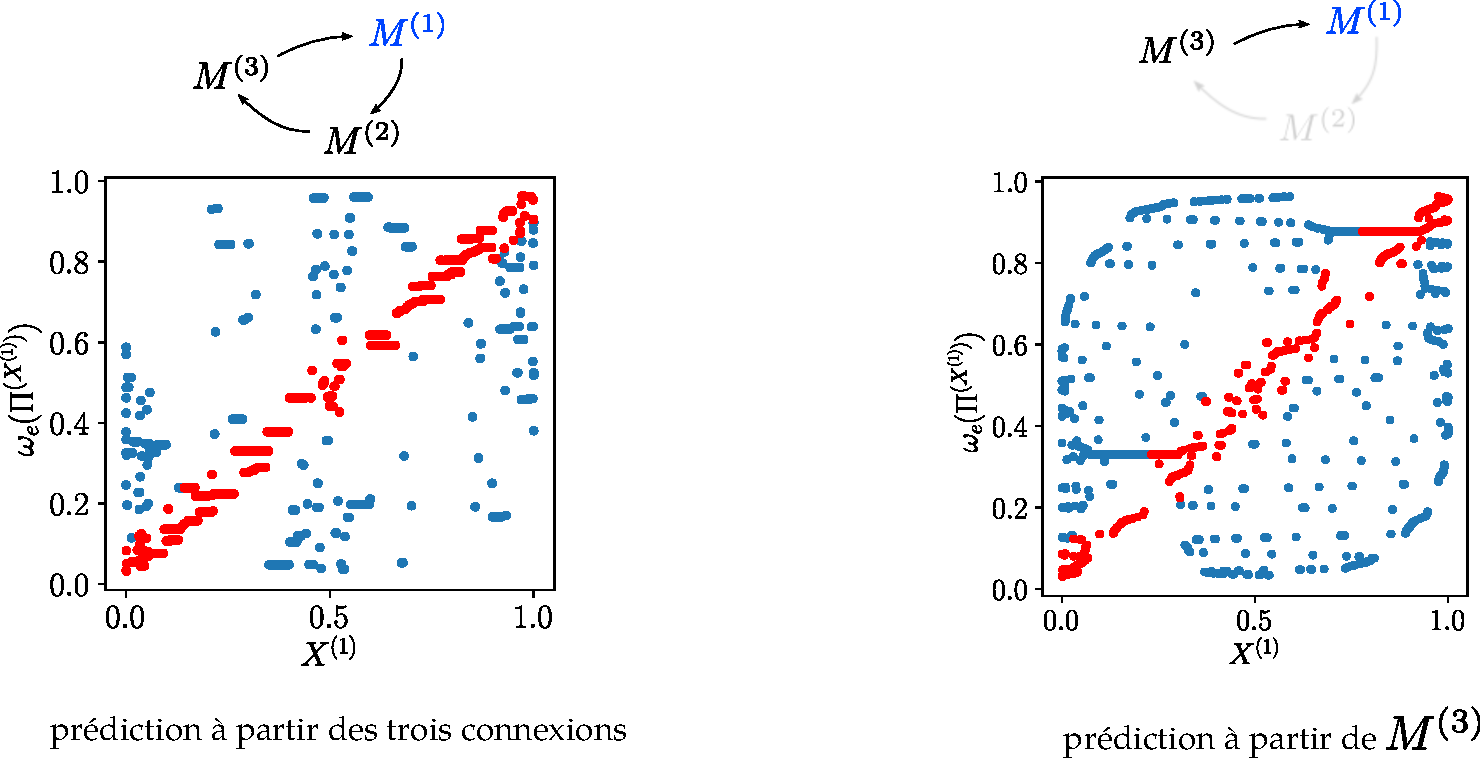
\includegraphics[width=0.9\textwidth]{loop/prediction_comparaison.pdf}
	\caption{\`A gauche, erreur de prédiction de l'entrée $\inpx\m{1}$ par l'architecture en boucle. Les points marqués en rouge représentent les valeurs correctement prédites à moins de $0.1$ près. 
	\`A droite, nous représentons l'erreur de prédiction réalisée à partir des mêmes poids de cartes en ne prenant en compte que $M\m{1}$ et $M\m{3}$. La prédiction est moins bien réalisée que dans le cas de gauche, ce qui montre que $M\m{2}$ a bien une influence sur le calcul du BMU de $M\m{1}$ via $M\m{2}$.
	\label{fig:pred_loop}}
\end{figure}

En figure~\ref{fig:pred_loop}, nous représentons la valeur de la prédiction dans l'architecture de trois cartes en fonction de l'entrée théorique $\inpx\m{1}$, comparée à une prédiction effectuée uniquement grâce à $M\m{3}$.
Nous remarquons d'abord que la prédiction est moins bien réalisée dans l'architecture en boucle, à gauche, que dans l'architecture avec rétroaction (cf. figure~\ref{fig:pred_cercle}).
Les valeurs prédites ayant une erreur de moins de 0.1 par rapport à leur entrée théorique, marquées par les points rouges, représentent seulement 55 \% des 2000 entrées présentées lors du test.
L'architecture en boucle n'a donc pas aussi bien appris le modèle d'entrées que dans le cas où les trois cartes sont connectées réciproquement, dans laquelle plus de 99 \% des valeurs sont prédites avec une erreur de moins de 0.1.
Cependant, la prédiction est mieux réalisée dans l'architecture en boucle que lorsque nous utilisons seulement $M\m{3}$ pour la prédiction.
Dans ce dernier cas, seules 40\% des entrées ont été correctement prédites par le couple de cartes~; l'erreur est globalement plus importante.
Cette observation montre qu'une carte conserve une influence à distance dans une architecture. Par contre, cette influence est très réduite par rapport à l'influence d'une connexion directe.

Nous pouvons conclure de ces deux observations que la disposition des connexions est un point important pour la construction d'architectures.
Les cartes ont peu d'influence à distance. Il faudra donc s'assurer que les modalités dont nous voulons apprendre les relations soient directement connectées. Cette observation est également prometteuse~: on peut ainsi envisager de traiter plusieurs flux d'information dans différentes parties d'une architecture, sans que le comportement d'une de ces parties n'affecte complètement les autres cartes.
A contrario, la présence de nombreuses connexions entre cartes semble moins limitante, l'architecture semblant être capable, grâce aux règles d'organisation, de moins prendre en compte les connexions venant d'une carte qui n'a pas de relation avec son entrée externe. 
Une possibilité d'étude de la connectivité serait également de construire des architectures adaptant leurs connexions au cours de l'apprentissage.

\section{Conclusion}

Ce chapitre de résultats présente une étude de l'organisation d'architectures de 2 et 3 cartes en une dimension.
Le but de ce chapitre est d'identifier les mécanismes d'organisation propres à CxSOM qui témoignent d'un apprentissage associatif du modèle d'entrées. Nous avons réalisé cette étude sur des données 1D afin de pouvoir en tracer une représentation facilement interprétable.

Nous avons d'abord observé que l'apprentissage du modèle d'entrées dans une architecture CxSOM est marqué par une organisation à deux échelles~: les poids externes se déplient sur l'espace d'entrée comme les poids d'une carte classique. Les poids contextuels se déplient sur des sous-régions de la carte, définies par la valeur de l'entrée externe, formant des motifs pseudo-périodiques~: la forme de ces périodes est similaire, mais varie en largeur spatiale et en amplitude. 
Cette organisation à deux échelles spatiales se retrouve dans l'organisation des BMU de chaque carte.
Ces derniers se disposent dans des zones distinctes, séparées par des zones mortes. 
Cette organisation permet d'encoder l'information sur tout le modèle d'entrées dans chacune des cartes. Nous avons en effet constaté qu'une zone de BMU se spécialise pour un intervalle de valeur du couple $(\inpx\m{1}, \inpx\m{2})$ ou $(\inpx\m{1}, \inpx\m{2}, \inpx\m{3})$ en 3D, représenté par $U$. L'apprentissage des relations entre entrées est alors marqué par le fait que $U$ est une position du BMU $\bmu$ dans chaque carte.

La notion de réponse à deux échelles se rapproche par ailleurs de certains modèles biologiques du cortex.
Cette organisation des cartes dépend des paramètres d'apprentissage, mais n'émerge que lorsque plusieurs points du modèle d'entrées partagent la même valeur sur une des modalités.
L'organisation en zones est caractéristique de l'apprentissage du modèle d'entrées par une architecture de cartes. Ce comportement est observé sur plusieurs jeux de données d'entrées jouets ainsi que réelles, sur des architectures de deux et trois cartes, et quel que soit le nombre de connexions entre cartes.


Nous avons ensuite constaté que l'encodage du modèle d'entrées complet dans chacune des cartes, effectué grâce à l'organisation à deux échelles, permet à l'architecture de prédire des valeurs d'entrées manquantes. Après apprentissage, une carte qui ne reçoit plus son entrée externe peut définir son BMU uniquement grâce à ses activités contextuelles.
Le poids externe du BMU peut être utilisé comme une valeur générée de la modalité qui n'a pas été présentée.
Dans ces tâches de prédiction, l'architecture CxSOM utilise le fait qu'elle ait encodé le modèle d'entrées de façon redondante entre les cartes. 
Cette capacité de prédiction est une application possible des architectures de cartes. Il s'agit également d'une façon d'évaluer l'apprentissage d'un modèle d'entrées par l'architecture lorsque ce modèle n'est pas connu en théorie.
La prédiction est un comportement qui différencie une carte simple ou une architecture hiérarchique de cartes d'une architecture non hiérarchique~: les modèles non hiérarchiques présentés au chapitre~\ref{chap:architectures} proposaient également cette capacité de prédiction. Nous voyons ici qu'il s'agit d'une capacité également permise par CxSOM. Dans notre cas, l'information n'est pas centralisée dans une carte associative. De plus, une prédiction peut-être réalisée par n'importe quelle carte grâce aux connexions non hiérarchiques, et s'appuie sur le même algorithme que celui utilisé lors des tests.

Maintenant que nous avons observé les comportements d'apprentissage dans des petites architectures de 2 et 3 cartes, une perspective principale d'étude de CxSOM est la construction d'architectures comportant plus de cartes.
Dans ces architectures, le choix des connexions entre cartes constitue un degré de liberté supplémentaire.
Nous avons présenté pour cela deux expériences questionnant l'influence des connexions entre les cartes.
Nous avons vu que des connexions distantes permettent toujours à l'architecture de cartes d'apprendre un modèle d'entrées. Cependant, lors de la prédiction, les cartes distantes de la carte prédictive ont moins d'influence que les cartes qui lui sont directement connectées.
Ensuite, nous avons observé que la présence de nombreuses entrées contextuelles amène les poids contextuels à s'organiser vers une valeur moyenne des entrées. Dans le cas où ces entrées seraient indépendantes au sein du modèle d'entrées, ce comportement de moyennage permettrait aux activités contextuelles de réduire leur contribution dans le calcul de l'activité globale~; le BMU ne prendrait alors en compte que les entrées qui présentent une dépendance.
Cependant, si $U$ est de grande dimension, tout couple de modalité $(\inpx\m{i}, \inpx\m{j})$ ne présentera que peu de dépendance, ce qui pourrait également entraîner ce comportement de moyennage. Ce n'est pas souhaitable, car nous voulons pouvoir extraire une représentation de $U$, même de grande dimension.

Plus généralement, il est difficilement souhaitable que chaque carte d'une architecture encode tout le modèle d'entrées lorsque $U$ est de dimension supérieure à 2.
Déjà lorsque $U$ est 2D, comme dans le patch $[0,1]^2$, la qualité de quantification vectorielle des entrées externes est significativement plus faible que celle obtenue sur un modèle $U$ 1D.
On attendrait plutôt de l'architecture qu'elle encode le modèle d'entrées de façon certes redondante, mais distribuée entre les cartes de l'architecture.
Cette distribution de la représentation de $U$ n'apparaît pas clairement dans les expériences sur deux et trois cartes, car les architectures sont encore trop petites. 
Cet aspect distribué de l'apprentissage sera un point à étudier sur des architectures de plus grande taille, et si besoin à corriger en adaptant les paramètres du modèle pour envisager un développement du modèle CxSOM à grande échelle. 
Il sera par exemple possible de jouer sur les connexions, les paramètres des cartes ou le calcul d'activité.

Ces constats soulèvent qu'il sera pertinent d'évaluer l'encodage du modèle d'entrées dans les cartes par des valeurs indicatrices.
La définition de valeurs indicatrices de cet encodage permettrait d'automatiser l'analyse des paramètres d'une architecture, de comparer des expériences entre elles et d'étudier des expériences dans lesquelles les tracés ne sont pas possibles à cause de la dimension des cartes et des entrées.
Ces indicateurs permettraient aussi d'étudier la distribution de l'encodage du modèle d'entrées au sein d'une architecture.
Nous étudierons quelques indicateurs d'analyse de l'encodage de $U$ par l'architecture au chapitre~\ref{chap:indicateur}.

Enfin, toutes ces expériences ont été menées sur des cartes 1D apprenant à représenter des données en une dimension. Ce cas de figure est rarement rencontré en pratique et il serait intéressant d'évaluer l'apprentissage sur des dimensions d'entrées supérieures. Pour une tâche de quantification vectorielle classique par une SOM, il est plus usuel d'utiliser des cartes en deux dimensions qui forment un bon compromis entre la capacité de quantification vectorielle rendue possible et le coût des calculs pendant l'apprentissage. Le passage de 1D à 2D n'est pas immédiat et pose de nombreuses questions quant à l'organisation des poids et la recherche de BMU par relaxation. 
Nous présenterons à ce propos au chapitre \ref{chap:analyse2D} des expériences préliminaires étudiant l'organisation d'une architecture de cartes en deux dimensions.

\ifSubfilesClassLoaded{
    \printbibliography
    %\externaldocument{../main.tex}   
}{}
\end{document}